%%
%% This is file `sample-sigconf-authordraft.tex',
%% generated with the docstrip utility.
%%
%% The original source files were:
%%
%% samples.dtx  (with options: `all,proceedings,bibtex,authordraft')
%% 
%% IMPORTANT NOTICE:
%% 
%% For the copyright see the source file.
%% 
%% Any modified versions of this file must be renamed
%% with new filenames distinct from sample-sigconf-authordraft.tex.
%% 
%% For distribution of the original source see the terms
%% for copying and modification in the file samples.dtx.
%% 
%% This generated file may be distributed as long as the
%% original source files, as listed above, are part of the
%% same distribution. (The sources need not necessarily be
%% in the same archive or directory.)
%%
%%
%% Commands for TeXCount
%TC:macro \cite [option:text,text]
%TC:macro \citep [option:text,text]
%TC:macro \citet [option:text,text]
%TC:envir table 0 1
%TC:envir table* 0 1
%TC:envir tabular [ignore] word
%TC:envir displaymath 0 word
%TC:envir math 0 word
%TC:envir comment 0 0
%%
%% The first command in your LaTeX source must be the \documentclass
%% command.
%%
%% For submission and review of your manuscript please change the
%% command to \documentclass[manuscript, screen, review]{acmart}.
%%
%% When submitting camera ready or to TAPS, please change the command
%% to \documentclass[sigconf]{acmart} or whichever template is required
%% for your publication.
%%
%%
% \documentclass[sigconf,authordraft]{acmart}
\documentclass[manuscript,review,anonymous]{acmart}
%%
%% \BibTeX command to typeset BibTeX logo in the docs
\AtBeginDocument{%
  \providecommand\BibTeX{{%
    Bib\TeX}}}

%% Rights management information.  This information is sent to you
%% when you complete the rights form.  These commands have SAMPLE
%% values in them; it is your responsibility as an author to replace
%% the commands and values with those provided to you when you
%% complete the rights form.
\setcopyright{acmlicensed}
\copyrightyear{2018}
\acmYear{2018}
\acmDOI{XXXXXXX.XXXXXXX}
%% These commands are for a PROCEEDINGS abstract or paper.
\acmConference[Conference acronym 'XX]{Make sure to enter the correct
  conference title from your rights confirmation email}{June 03--05,
  2018}{Woodstock, NY}
%%
%%  Uncomment \acmBooktitle if the title of the proceedings is different
%%  from ``Proceedings of ...''!
%%
%%\acmBooktitle{Woodstock '18: ACM Symposium on Neural Gaze Detection,
%%  June 03--05, 2018, Woodstock, NY}
\acmISBN{978-1-4503-XXXX-X/2018/06}


%%
%% Submission ID.
%% Use this when submitting an article to a sponsored event. You'll
%% receive a unique submission ID from the organizers
%% of the event, and this ID should be used as the parameter to this command.
%%\acmSubmissionID{123-A56-BU3}

%%
%% For managing citations, it is recommended to use bibliography
%% files in BibTeX format.
%%
%% You can then either use BibTeX with the ACM-Reference-Format style,
%% or BibLaTeX with the acmnumeric or acmauthoryear sytles, that include
%% support for advanced citation of software artefact from the
%% biblatex-software package, also separately available on CTAN.
%%
%% Look at the sample-*-biblatex.tex files for templates showcasing
%% the biblatex styles.
%%

%%
%% The majority of ACM publications use numbered citations and
%% references.  The command \citestyle{authoryear} switches to the
%% "author year" style.
%%
%% If you are preparing content for an event
%% sponsored by ACM SIGGRAPH, you must use the "author year" style of
%% citations and references.
%% Uncommenting
%% the next command will enable that style.
%%\citestyle{acmauthoryear}


%%
%% end of the preamble, start of the body of the document source.
\usepackage{booktabs,tabularx,array,subcaption,float}
\usepackage{amsmath} % For mathematical environments
\usepackage{enumitem} % For customizing lists
\usepackage{tcolorbox}
\usepackage{lipsum}
\usepackage{xcolor}
\usepackage{verbatim} % For \begin{comment}...\end{comment}

% ---- Revision tracking ----
\definecolor{revcolor}{rgb}{0.8,0,0}
\newcommand{\revstart}{\color{revcolor}}  % start revised block
\newcommand{\revend}{\color{black}}       % end revised block
\newcommand{\rev}[1]{\textcolor{revcolor}{#1}}  % inline revised text
% To disable all highlighting, uncomment the following:
% \renewcommand{\revstart}{}
% \renewcommand{\revend}{}
% \renewcommand{\rev}[1]{#1}

% Define a command for small italic text
\newcommand{\smallitalic}[1]{{\small\textit{#1}}}
\newcommand{\strategy}[1]{{\textit{#1}}}
\begin{document}

%%
%% The "title" command has an optional parameter,
%% allowing the author to define a "short title" to be used in page headers.
\title{Investigating Questioning Strategies for Robot Learning by Asking in Household Tasks}

%%
%% The "author" command and its associated commands are used to define
%% the authors and their affiliations.
%% Of note is the shared affiliation of the first two authors, and the
%% "authornote" and "authornotemark" commands
%% used to denote shared contribution to the research.
% \author{Ben Trovato}
% \authornote{Both authors contributed equally to this research.}
% \email{trovato@corporation.com}
% \orcid{1234-5678-9012}
% \author{G.K.M. Tobin}
% \authornotemark[1]
% \email{webmaster@marysville-ohio.com}
% \affiliation{%
%   \institution{Institute for Clarity in Documentation}
%   \city{Dublin}
%   \state{Ohio}
%   \country{USA}
% }

% \author{Lars Th{\o}rv{\"a}ld}
% \affiliation{%
%   \institution{The Th{\o}rv{\"a}ld Group}
%   \city{Hekla}
%   \country{Iceland}}
% \email{larst@affiliation.org}

% \author{Valerie B\'eranger}
% \affiliation{%
%   \institution{Inria Paris-Rocquencourt}
%   \city{Rocquencourt}
%   \country{France}
% }

% \author{Aparna Patel}
% \affiliation{%
%  \institution{Rajiv Gandhi University}
%  \city{Doimukh}
%  \state{Arunachal Pradesh}
%  \country{India}}

% \author{Huifen Chan}
% \affiliation{%
%   \institution{Tsinghua University}
%   \city{Haidian Qu}
%   \state{Beijing Shi}
%   \country{China}}

% \author{Charles Palmer}
% \affiliation{%
%   \institution{Palmer Research Laboratories}
%   \city{San Antonio}
%   \state{Texas}
%   \country{USA}}
% \email{cpalmer@prl.com}

% \author{John Smith}
% \affiliation{%
%   \institution{The Th{\o}rv{\"a}ld Group}
%   \city{Hekla}
%   \country{Iceland}}
% \email{jsmith@affiliation.org}

% \author{Julius P. Kumquat}
% \affiliation{%
%   \institution{The Kumquat Consortium}
%   \city{New York}
%   \country{USA}}
% \email{jpkumquat@consortium.net}

\author{Yuanda Hu}
\affiliation{%
  \institution{College of Design and Innovation, Tongji University}
  \city{Shanghai}
  \country{China}
}
\email{ydhu@tongji.edu.cn}

\author{Jiani Hou}
\affiliation{%
  \institution{School of Design, Southern University of Science and Technology}
  \city{Shenzhen}
  \country{China}
}

\author{Dai Shi}
\affiliation{%
  \institution{College of Design and Innovation, Tongji University}
  \city{Shanghai}
  \country{China}
}

\author{Suming Li}
\affiliation{%
  \institution{College of Architecture and Urban Planning, Tongji University}
  \city{Shanghai}
  \country{China}
}
\email{SunnyMing@tongji.edu.cn}

\author{Yujie Qiu}
\affiliation{%
  \institution{School of Mechanical and Manufacturing Engineering, University of New South Wales}
  \city{Sydney}
  \state{NSW}
  \country{Australia}
}
\email{z5637231@ad.unsw.edu.au}

\author{Yate Ge}
\affiliation{%
  \institution{College of Design and Innovation, Tongji University}
  \city{Shanghai}
  \country{China}
}
\email{geyate@tongji.edu.cn}

\author{Qi Wang}
\affiliation{%
  \institution{College of Design and Innovation, Tongji University}
  \city{Shanghai}
  \country{China}
}

\author{Xiaohua Sun}
\affiliation{%
  \institution{School of Design, Southern University of Science and Technology}
  \city{Shenzhen}
  \state{Guangdong}
  \country{China}
}

\author{Weiwei Guo}
\affiliation{%
  \institution{College of Design and Innovation, Tongji University}
  \city{Shanghai}
  \country{China}
}


%%
%% By default, the full list of authors will be used in the page
%% headers. Often, this list is too long, and will overlap
%% other information printed in the page headers. This command allows
%% the author to define a more concise list
%% of authors' names for this purpose.
\renewcommand{\shortauthors}{Trovato et al.}

%%
%% The abstract is a short summary of the work to be presented in the
%% article.
\begin{abstract}
{\revstart
How should robots ask questions to learn household preferences efficiently? While prior work has explored active questioning in human--robot interaction, the impact of different questioning \textit{strategies} on objective task performance remains unquantified. We address this gap through three contributions. First, in a formative human--human study, we identify three distinct questioning patterns people naturally exhibit when teaching household tasks: \textit{Direct Querying} (item-by-item), \textit{User-Preference-First} (eliciting general rules before specific actions), and \textit{Parallel Exploration} (interleaving actions with rule induction). Second, we formalize these patterns as three questioning design patterns---Action-Oriented, Preference-Eliciting, and Preference-Induction---composed into four questioning strategies within a structured preference learning framework. Third, through a large-scale simulation study (102 household episodes, budget 1--10), we provide the first quantitative evidence that strategy choice measurably affects placement accuracy: the User-Preference-First strategy achieves 69.8\% unseen-object accuracy at budget~5, outperforming Direct Querying (58.7\%) by +11.1 percentage points, because top-down preference elicitation produces category-level rules that generalize to novel objects. Bottom-up induction offers no significant advantage over direct querying, and adaptive strategy switching does not outperform the simpler preference-first heuristic. These findings demonstrate that questioning strategy design is a critical and quantifiable factor in robot Learning by Asking.
% TODO: Add Study 2 (user study) findings when available.
\revend}
\end{abstract}

%%
%% The code below is generated by the tool at http://dl.acm.org/ccs.cfm.
%% Please copy and paste the code instead of the example below.
% %%
% \begin{CCSXML}

% <ccs2012>
%  <concept>
%   <concept_id>00000000.0000000.0000000</concept_id>
%   <concept_desc>Do Not Use This Code, Generate the Correct Terms for Your Paper</concept_desc>
%   <concept_significance>500</concept_significance>
%  </concept>
%  <concept>
%   <concept_id>00000000.00000000.00000000</concept_id>
%   <concept_desc>Do Not Use This Code, Generate the Correct Terms for Your Paper</concept_desc>
%   <concept_significance>300</concept_significance>
%  </concept>
%  <concept>
%   <concept_id>00000000.00000000.00000000</concept_id>
%   <concept_desc>Do Not Use This Code, Generate the Correct Terms for Your Paper</concept_desc>
%   <concept_significance>100</concept_significance>
%  </concept>
%  <concept>
%   <concept_id>00000000.00000000.00000000</concept_id>
%   <concept_desc>Do Not Use This Code, Generate the Correct Terms for Your Paper</concept_desc>
%   <concept_significance>100</concept_significance>
%  </concept>
% </ccs2012>
% \end{CCSXML}

\begin{CCSXML}
<ccs2012>
   <concept>
       <concept_id>10003120.10003121</concept_id>
       <concept_desc>Human-centered computing~Human computer interaction (HCI)</concept_desc>
       <concept_significance>500</concept_significance>
       </concept>
   <concept>
       <concept_id>10010147.10010178.10010199.10010204</concept_id>
       <concept_desc>Computing methodologies~Robotic planning</concept_desc>
       <concept_significance>300</concept_significance>
       </concept>
   <concept>
       <concept_id>10010147.10010178.10010179.10010181</concept_id>
       <concept_desc>Computing methodologies~Discourse, dialogue and pragmatics</concept_desc>
       <concept_significance>300</concept_significance>
       </concept>
 </ccs2012>
\end{CCSXML}

\ccsdesc[500]{Human-centered computing~Human computer interaction (HCI)}
\ccsdesc[300]{Computing methodologies~Robotic planning}
\ccsdesc[300]{Computing methodologies~Discourse, dialogue and pragmatics}
\ccsdesc[500]{Human-centered computing~Empirical studies in HCI}

% \ccsdesc[500]{Do Not Use This Code~Generate the Correct Terms for Your Paper}
% \ccsdesc[300]{Do Not Use This Code~Generate the Correct Terms for Your Paper}
% \ccsdesc{Do Not Use This Code~Generate the Correct Terms for Your Paper}
% \ccsdesc[100]{Do Not Use This Code~Generate the Correct Terms for Your Paper}

%%
%% Keywords. The author(s) should pick words that accurately describe
%% the work being presented. Separate the keywords with commas.
% \keywords{Do, Not, Us, This, Code, Put, the, Correct, Terms, for,
%   Your, Paper}
\keywords{\rev{Human-Robot Interaction, Questioning Strategies, Preference Learning, Large Language Models, Household Tasks}}

%% A "teaser" image appears between the author and affiliation
%% information and the body of the document, and typically spans the
%% page.
\begin{teaserfigure}
  
\includegraphics[width=\textwidth]{teaser}
  \caption{\rev{We study how questioning strategies affect robot learning of household preferences. Our work (1) identifies three distinct questioning patterns in human teaching, (2) formalizes them as questioning design patterns within a structured preference learning framework, and (3) quantifies their impact on placement accuracy through large-scale simulation, showing that top-down preference elicitation significantly outperforms item-by-item querying on novel objects.}}
  % TODO: Update teaser figure to reflect new system architecture
  \Description{Enjoying the baseball game from the third-base
  seats. Ichiro Suzuki preparing to bat.}
  \label{fig:teaser}
\end{teaserfigure}

\received{20 February 2007}
\received[revised]{12 March 2009}
\received[accepted]{5 June 2009}

%%
%% This command processes the author and affiliation and title
%% information and builds the first part of the formatted document.
\maketitle

\section{Introduction}
{\revstart

Household tasks are inherently open-ended and shaped by diverse user preferences, making it difficult for robots to reliably align with human expectations~\cite{wu2023tidybot,nasiriany2024robocasa}. Beyond perceiving the physical environment, effective assistance requires robots to proactively acquire and adapt to individual preferences~\cite{zheng2019personalized,lawley2024val}. Learning by Asking (LBA) provides a natural and efficient mechanism to reduce uncertainty, clarify intentions, and gradually build common ground with users~\cite{biyik2019asking,6padmakumar2022teach,8leusmann2025investigating}. For example, in an organizing task, a robot might ask about each object in turn---``Should this book go on the shelf?''---or instead begin with a broader question such as ``Do you usually separate study materials from daily supplies?''. These two approaches reflect fundamentally different \textit{questioning strategies}, and prior work in human teaching and collaboration shows that how questions are organized strongly shapes communication efficiency and perceived control~\cite{cakmak2012designing,mutlu2009footing}.

A substantial body of work has examined active question-asking in robotics as a computational mechanism to reduce task ambiguity~\cite{cakmak2012designing,biyik2019asking,habibian2022here}. However, these approaches typically target simple settings---evaluating whether a single clarification resolves ambiguity or asking once to learn about a novel object~\cite{5ramrakhya2025grounding,7uehara2024learning,12biyik2019asking}. While such atomic questioning is effective in isolation, naively extending it to long-horizon household tasks results in unstructured, repetitive dialogue that degrades user experience and fails to capture transferable preferences~\cite{oviatt2006human,kosch2023survey}. A deeper limitation lies in the emphasis on \textit{how} to ask (e.g., algorithmic follow-ups) while neglecting \textit{when, in what order, and for what purpose} to ask~\cite{tyshka2023interactive,hu2024designing}. Moreover, existing evaluations focus almost exclusively on subjective user perceptions, leaving a critical question unanswered: \textbf{does the choice of questioning strategy measurably affect task performance?}

This paper addresses three research questions:

\begin{itemize}[leftmargin=*]
    \item \textbf{RQ1}: In household teaching scenarios, do humans naturally exhibit distinguishable questioning patterns?
    \item \textbf{RQ2}: Can these patterns be formalized as composable dialogue policies and deployed within a structured preference learning framework?
    \item \textbf{RQ3}: Do different questioning strategies produce measurably different outcomes in \textit{objective task performance}---specifically, in the accuracy with which learned preferences generalize to novel objects?
\end{itemize}

To answer RQ1, we conducted a formative human--human study in which participants taught household tasks through dialogue. We identified three distinct questioning patterns: \textit{Direct Querying} (item-by-item), \textit{User-Preference-First} (establishing general rules before addressing specific items), and \textit{Parallel Exploration} (interleaving concrete actions with periodic rule induction). For RQ2, we formalized these patterns as three questioning design patterns---Action-Oriented (AO), Preference-Eliciting (PE), and Preference-Induction (PI)---and composed them into four questioning strategies within a structured preference learning framework. Unlike end-to-end LLM approaches that retain only raw dialogue history, our framework maintains a structured preference state that explicitly separates confirmed placements, category-level rules, and negative evidence, enabling hierarchical reasoning during final placement. For RQ3, we conducted a large-scale simulation study across 102 household episodes with question budgets ranging from 1 to 10, comparing four strategies and two baselines (No Question, Raw LLM).

Our results demonstrate that strategy choice has a substantial and quantifiable impact on task performance. The User-Preference-First strategy (UPF) achieves 69.8\% unseen-object accuracy at budget~5, outperforming Direct Querying's 58.7\% by +11.1 percentage points---because top-down preference elicitation produces category-level rules that generalize to novel objects. In contrast, the bottom-up Parallel Exploration strategy, which interleaves actions with periodic rule induction, offers no significant advantage over direct querying, as induction requires multiple prior turns to accumulate evidence, reducing budget efficiency. Adaptive strategy switching (Hybrid-All) does not outperform the simpler UPF heuristic. These findings provide the first quantitative evidence that questioning strategy design is a critical factor in robot Learning by Asking.

Our key contributions are:
\begin{enumerate}
  \item Identifying and empirically validating three distinct questioning patterns in household teaching through a formative human--human study;
  \item Designing a structured preference learning framework that formalizes these patterns as questioning design patterns (AO, PE, PI), composed into four questioning strategies, supported by structured state representation and evidence-based placement planning;
  \item Providing the first large-scale quantitative evaluation of questioning strategies in household preference learning, demonstrating that top-down preference elicitation significantly outperforms item-by-item and bottom-up approaches on generalization to novel objects.
  % TODO: Add contribution 4 (user study) when Study 2 is complete.
\end{enumerate}
\revend}

\section{Related Work}
\subsection{Robot Learning in Household Tasks}

In household tasks, successful robot performance often hinges on capturing deeper information that reflects user characteristics and contextual variations, which cannot be fully encoded in advance \cite{zhong2021gap}. To address this, researchers have explored learning approaches that acquire user preferences or constraints through dynamic human–robot interaction. Based on who initiates the exchange, existing work can be divided into three categories: human-initiated teaching, interactive learning, and robot-initiated learning.

Human-initiated teaching transfers task knowledge or preferences through demonstrations or explicit instructions, focusing on extracting useful information from user input. Examples include trajectory imitation for complex operations \cite{tsuji2025survey,hussein2017imitation,wake2024gpt}  or combining language with demonstrations to teach new skills \cite{she2014teaching}. To support such methods, the research community has developed large-scale simulation platforms and multi-modal datasets—for example, RoboCasa \cite{nasiriany2024robocasa} offers a scalable environment for everyday task simulation, while the NatSGD dataset provides speech, gesture, and demonstration data to facilitate learning in natural human–robot interaction scenarios \cite{shrestha2024natsgd}.

Interactive learning emphasizes bidirectional exchange, where robots and users iteratively build task understanding through dialogue, corrections, and demonstrations. Methods such as Interactive Task Learning  and dialogue-based lifelong learning explore how to incrementally integrate new information while retaining prior knowledge \cite{tyshka2023interactive,reimann2024survey,schmidt2018survey,luo2019learning,zheng2019personalized,lawley2024val} .

Robot-initiated learning reduces uncertainty by actively posing questions or probing. A typical method is active learning, which centers on selecting the most valuable questions based on uncertainty or utility functions, while balancing information gain against the burden placed on the human respondent. For example, some studies propose questioning strategies that both reveal the current knowledge of the robot and remain easy for humans to interpret \cite{habibian2022here}, as well as user-friendly active querying methods that are easy to answer\cite{biyik2019asking}. Other approaches attempt to learn from observing user actions and feedback \cite{wu2023tidybot}. However, when relying solely on robot-driven learning without user involvement, these methods remain insufficient to fully capture the deeper-level information required for task completion.

Overall, each approach has distinct strengths: human teaching depends on high-quality demonstrations, interactive learning builds on long-term accumulation, and robot-initiated learning emphasizes efficient exploration. For long-duration household tasks such as organizing refrigerators or arranging objects, multi-turn robot questioning offers a natural and effective way to uncover deeper information \cite{hunt2024survey}. Therefore, we focuses on the study and application of multi-turn active questioning strategies in household settings.

\subsection{Learning By Asking in Human–Robot Interaction}
In human robot interaction research, learning by asking has been emerging as an important approach to endowing robots with intelligent behaviors. Its core idea is to enable robots to actively acquire information by posing questions~\cite{hu2025task,shen2025elba}.Existing active learning strategies can be broadly categorized into three types: 
(i) ambiguity-resolution questioning, where robots ask specific questions (e.g., ``Which cup?'' or ``Where exactly is `next to'?'' ) to clarify referential or semantic ambiguities in instructions~\cite{3ren2023robots,4andukuri2024star,5ramrakhya2025grounding,6padmakumar2022teach}; 
(ii) knowledge-completion questioning, where robots seek missing information during task planning (e.g., ``I don't know what is inside this drawer'')~\cite{hu2025task,7uehara2024learning}; 
and (iii) curiosity-driven exploratory questioning, where robots investigate unknown objects or areas to expand their knowledge base~\cite{8leusmann2025investigating,9carter2022you,10leusmann2025developing,11scialom2019ask}.

However, these methods typically target relatively simple task settings~\cite{7uehara2024learning,12biyik2019asking,13gonzalez2018analyzing}, such as evaluating whether a single clarification resolves ambiguity~\cite{5ramrakhya2025grounding,7uehara2024learning} or asking once to acquire knowledge about a novel object~\cite{12biyik2019asking,shen2019learning}. While such atomic questioning strategies are effective in isolated cases, naively extending them to long-horizon tasks often results in unstructured questioning, which can degrade user experience, reduce interaction efficiency, and create a mechanical impression. This highlights the need for macro-level planning in human--robot question--answering~\cite{oviatt2006human,kosch2023survey,tyshka2023interactive}. The underlying limitation lies in an emphasis on how to ask (e.g., algorithmic follow-ups) while neglecting when, in what order, and for what purpose to ask~\cite{tyshka2023interactive,hu2024designing}. Studies on cognitive load further show that frequent attentional shifts can impair cognitive performance~\cite{kosch2023survey}.

By contrast, the dialogue systems community has demonstrated that strategic questioning is key to managing multi-turn tasks, as it reduces cognitive burden and improves efficiency~\cite{stivers2010overview,kwan2023survey}. For instance, Stivers' analysis shows that macro-level planning of polar and wh-question sequences (e.g., prioritizing confirmations) optimizes information gathering~\cite{stivers2010overview}, while reinforcement learning approaches in dialogue rely on policies to handle long sequences~\cite{kwan2023survey}.

In summary, while strategy-driven questioning has been shown to enhance coherence and effectiveness in multi-turn dialogue systems, HRI research has largely focused on optimizing individual questions, with limited attention to macro-level organization in long-horizon tasks~\cite{hu2024designing}. \rev{Critically, existing evaluations of questioning in HRI rely almost exclusively on subjective measures (e.g., perceived workload, curiosity, or trust), leaving open the question of whether different questioning strategies produce measurably different \textit{task outcomes}. This paper addresses this gap by combining human-derived questioning patterns with a structured preference learning framework and providing the first large-scale quantitative evaluation of their impact on placement accuracy.}




\subsection{Dialogue and Questioning Strategies}
Research on questioning in dialogue can generally be divided into two categories: theoretical studies and applied explorations in human–robot interaction. The former provide a methodological foundation for understanding how to ask, while the latter demonstrate how these methods can be implemented in practical systems.

Theoretical studies mainly based on education and qualitative research methodology. Educational research emphasizes the relationship between cognitive levels of questioning and learning outcomes, examining how teachers design questions to foster deeper thinking and self-monitoring in students~\cite{redfield1981meta,tofade2013best}. Empirical evidence and teaching practices further suggest that strategies such as waiting time, follow-up questioning, and self-questioning training play an important role in classroom effectiveness~\cite{redfield1981meta,tofade2013best}. Qualitative research has developed a set of operational tools to support probing for deeper information ~\cite{robinson2023probing,balza2022effective,dejonckheere2019semistructured}. For example, probing studies identify different types of follow-up questions and highlight their role in building trust, avoiding bias, and ensuring data credibility~\cite{robinson2023probing}; while semi-structured interviewing distills key skills for designing and conducting follow-up questions in research practice~\cite{dejonckheere2019semistructured}. Together, these theoretical and methodological contributions provide important insights for the design of questioning strategies in HRI.

In HRI research, some studies have directly drawn on these theories to design questioning mechanisms for dialogue agents or robots~\cite{hu2024designing,cakmak2012designing,habibian2022here}. Other work explores the generation of human-like questions under uncertainty~\cite{shin2023uncertainty} and the use of questioning strategies to improve information gathering~\cite{hu2025task}. A further line of research frames questioning as an interaction strategy that balances task efficiency with human workload. Typical scenarios include gradually acquiring knowledge through interaction with humans.\cite{adamson2021we} or requesting expert assistance at appropriate times during embodied tasks \cite{singh2022ask4help}. These studies model questioning as a decision-making problem, aiming to balance task performance with the quality of human–robot collaboration.

Despite these advances, limitations remain when applying such methods to multi-turn questioning in real-world HRI scenarios. In particular, for long-duration household tasks, there is still little guidance on how robots might employ more natural questioning strategies to acquire and update user preferences, thereby uncovering deeper-level information. To address this gap, this paper observes human face-to-face teaching in domestic settings, identifies natural questioning patterns, and maps them onto robot-specific questioning strategies for HRI.

\subsection{\rev{LLMs for Interactive Robot Learning}}
{\revstart
With the rapid development of large language models (LLMs) and vision--language models (VLMs), robots have made significant progress in perception, reasoning, and task execution in open environments. Representative works such as PaLM-E~\cite{driess2023palm} and RT-2~\cite{zitkovich2023rt} demonstrate that VLMs can unify multimodal perception and language reasoning, while related surveys~\cite{ma2024survey,zeng2023large} highlight LLMs/VLMs as a key technological foundation for natural interaction and long-horizon planning in embodied intelligence.

However, existing research often treats LLMs as black-box generators directly applied to instruction parsing or action planning. For example, Instruct2Act~\cite{huang2023instruct2act} and Manual2Skill~\cite{tie2025manual2skill} showcase the effectiveness of LLMs in understanding complex instructions and executing long-horizon tasks, but do not address controllable questioning or structured preference extraction. Some efforts have explored asking for help under uncertainty~\cite{3ren2023robots,5ramrakhya2025grounding} or leveraging questions to improve performance in specific tasks~\cite{4andukuri2024star,shen2025elba}, yet these remain limited to isolated scenarios. In household organization, TidyBot~\cite{wu2023tidybot} demonstrates that LLMs can generalize object placement from a few examples, but relies on passive observation rather than active questioning.

A key design question is whether to retain raw dialogue history or extract structured intermediate representations. End-to-end LLM approaches that read the full conversation are simple but suffer from context limitations, information loss, and difficulty enforcing evidence hierarchies~\cite{tyshka2023interactive}. In contrast, structured state representations---where confirmed actions, category-level rules, and negative evidence are explicitly separated---enable more consistent and controllable multi-turn reasoning. Our work adopts the structured approach and empirically validates its advantage over end-to-end LLM baselines through controlled experiments.
\revend}

\section{Human–Human Study of Questioning Patterns}
Previous research has highlighted the critical role of questioning in aligning user preferences and facilitating collaboration~\cite{cakmak2012designing,hu2024designing}. However, it remains unclear whether people employ systematic patterns of questioning when performing such tasks. For example, a learner might directly ask for overarching preferences at the outset, or alternatively, infer and confirm preferences incrementally based on contextual cues. To investigate this, we conducted a \textit{Human--Human Interaction (HHI) study} focusing on representative household tasks. In each session, one participant acted as the ``teacher,'' responding according to their personal habits and preferences, while the other participant played the role of the ``learner,'' who could only acquire task-relevant knowledge by asking questions. By analyzing these dialogues, our goal was to uncover whether the sequences of questions exhibited recognizable structures, and if so, how these structures manifested as distinct patterns across different stages of the task---namely, eliciting preferences, guiding operational steps, and accomplishing the final goal.

\subsection{Participants}
We first recruited participants through a screening questionnaire, which asked them to report the number of times they had completed the tasks of ``organizing a refrigerator'' and ``mixing cocktails'' in the past ten months, as well as to provide basic demographic information and self-rated task familiarity. We collected 34 valid responses and subsequently expanded the recruitment, resulting in a total of 40 volunteers from a university community. All participants received monetary compensation. 

Based on the questionnaire results, participants who had performed a given task more than three times in the past ten months were classified as \textit{task-familiar}, while those who had performed it once or fewer times were classified as \textit{task-unfamiliar}. In the experimental design, task-familiar participants were assigned the role of \textit{teacher}, responsible for answering questions according to their own habits and preferences. Task-unfamiliar participants were assigned the role of \textit{learner}, who could only acquire task-relevant information by asking questions. To ensure balanced comparisons, we adopted a pairing strategy, randomly assigning each teacher to a learner. In total, 14 dyads (28 participants) were invited to take part in the formal experiment. 

Participants had a mean age of 22 years and were either undergraduate or graduate students with normal or corrected-to-normal vision. All participants provided informed consent prior to the study. Teachers were instructed to familiarize themselves with the experimental environment and to imagine it as part of their everyday household setting, so as to naturally reproduce their authentic operational habits and preferences.


\subsection{Procedure}
We selected two representative household tasks for this study: organizing a refrigerator and mixing cocktails. Following prior work~\cite{dai2024think}~\cite{racca2018active}, household service tasks can generally be divided into two categories: (1) tasks that primarily aim to achieve a final desired state, such as organizing storage spaces or arranging items, and (2) tasks that emphasize procedural steps and order, such as cooking or cocktail preparation. The refrigerator organization task centers on achieving a coherent and efficient arrangement of items, while the order of specific steps is relatively flexible. In contrast, cocktail mixing requires sequential completion of subtasks with fixed ratios and procedures. By selecting these two tasks, we aimed to capture questioning strategies across different task structures. 

In the experiment, participants were paired to complete the tasks collaboratively. The \textit{learner} could only obtain information through asking questions and had to execute the physical operations accordingly. The \textit{teacher}, in turn, answered questions based on their own habits and preferences but did not perform any physical actions. We emphasized that teachers should rely solely on the verbal modality, without using demonstration-based teaching or collaborative manipulation. Thus, learners were required to depend entirely on questioning to gradually infer the teacher’s rules or preferences and proceed with the task. 

Before the main trials, teachers were instructed to familiarize themselves with the experimental environment and to imagine it as part of their everyday household setting, enabling them to reproduce their authentic habits naturally. Each pair of participants then completed two tasks in sequence: first organizing the refrigerator, followed by mixing cocktails. The completion of each task was determined by the participants themselves, who informed the experimenter once they considered the task finished. To ensure comprehensive analysis, we recorded the entire process with a GoPro Hero 9 camera, capturing both audio and video of the participants’ questioning, responses, and task operations. Figure~\ref{fig:procedure} illustrates two example interactions from the experiment.

\begin{figure}[t]
  \centering
  \includegraphics[width=\linewidth]{img/3.2.png}
  \caption{Illustration of the experimental procedure. 
  Left: In the refrigerator organization task, the learner asks about the teacher’s organizing principles (e.g., ``Do you organize by beverage type or by box height?''). 
  Right: In the cocktail mixing task, the learner queries the teacher’s preferences (e.g., ``Do you like fruit-based drinks?'').}
  \label{fig:procedure}
\end{figure}

\subsection{Hierarchical Coding Framework}
To systematically analyze how humans ask questions in task-oriented dialogues, we developed a hierarchical coding framework with three levels, \rev{following an iterative thematic analysis approach~\cite{braun2006using}}. At the first level, each question is annotated by its \textit{knowledge type} (Knowledge-level Annotation). At the second level, questions are further coded according to their \textit{interactional intent} (Intent-level Coding). At the third level, sequences of questions are analyzed to identify recurring \textit{patterns} across dialogues (Pattern Identification). Figure~\ref{fig:annotation-pipeline} illustrates this process, showing how raw dialogues are progressively annotated and abstracted to yield the questioning patterns.

\rev{Two researchers independently coded all 28 dialogue transcripts across both levels. Inter-rater reliability was assessed using Cohen's $\kappa$ at each coding level: knowledge-level annotation achieved $\kappa = $~\textbf{TODO} and intent-level coding achieved $\kappa = $~\textbf{TODO}. Disagreements were resolved through discussion until consensus was reached; the final codebook was reviewed and validated by two additional researchers.}
% TODO: Fill in actual Cohen's kappa values from coding data.

\begin{figure}[t]
  \centering
  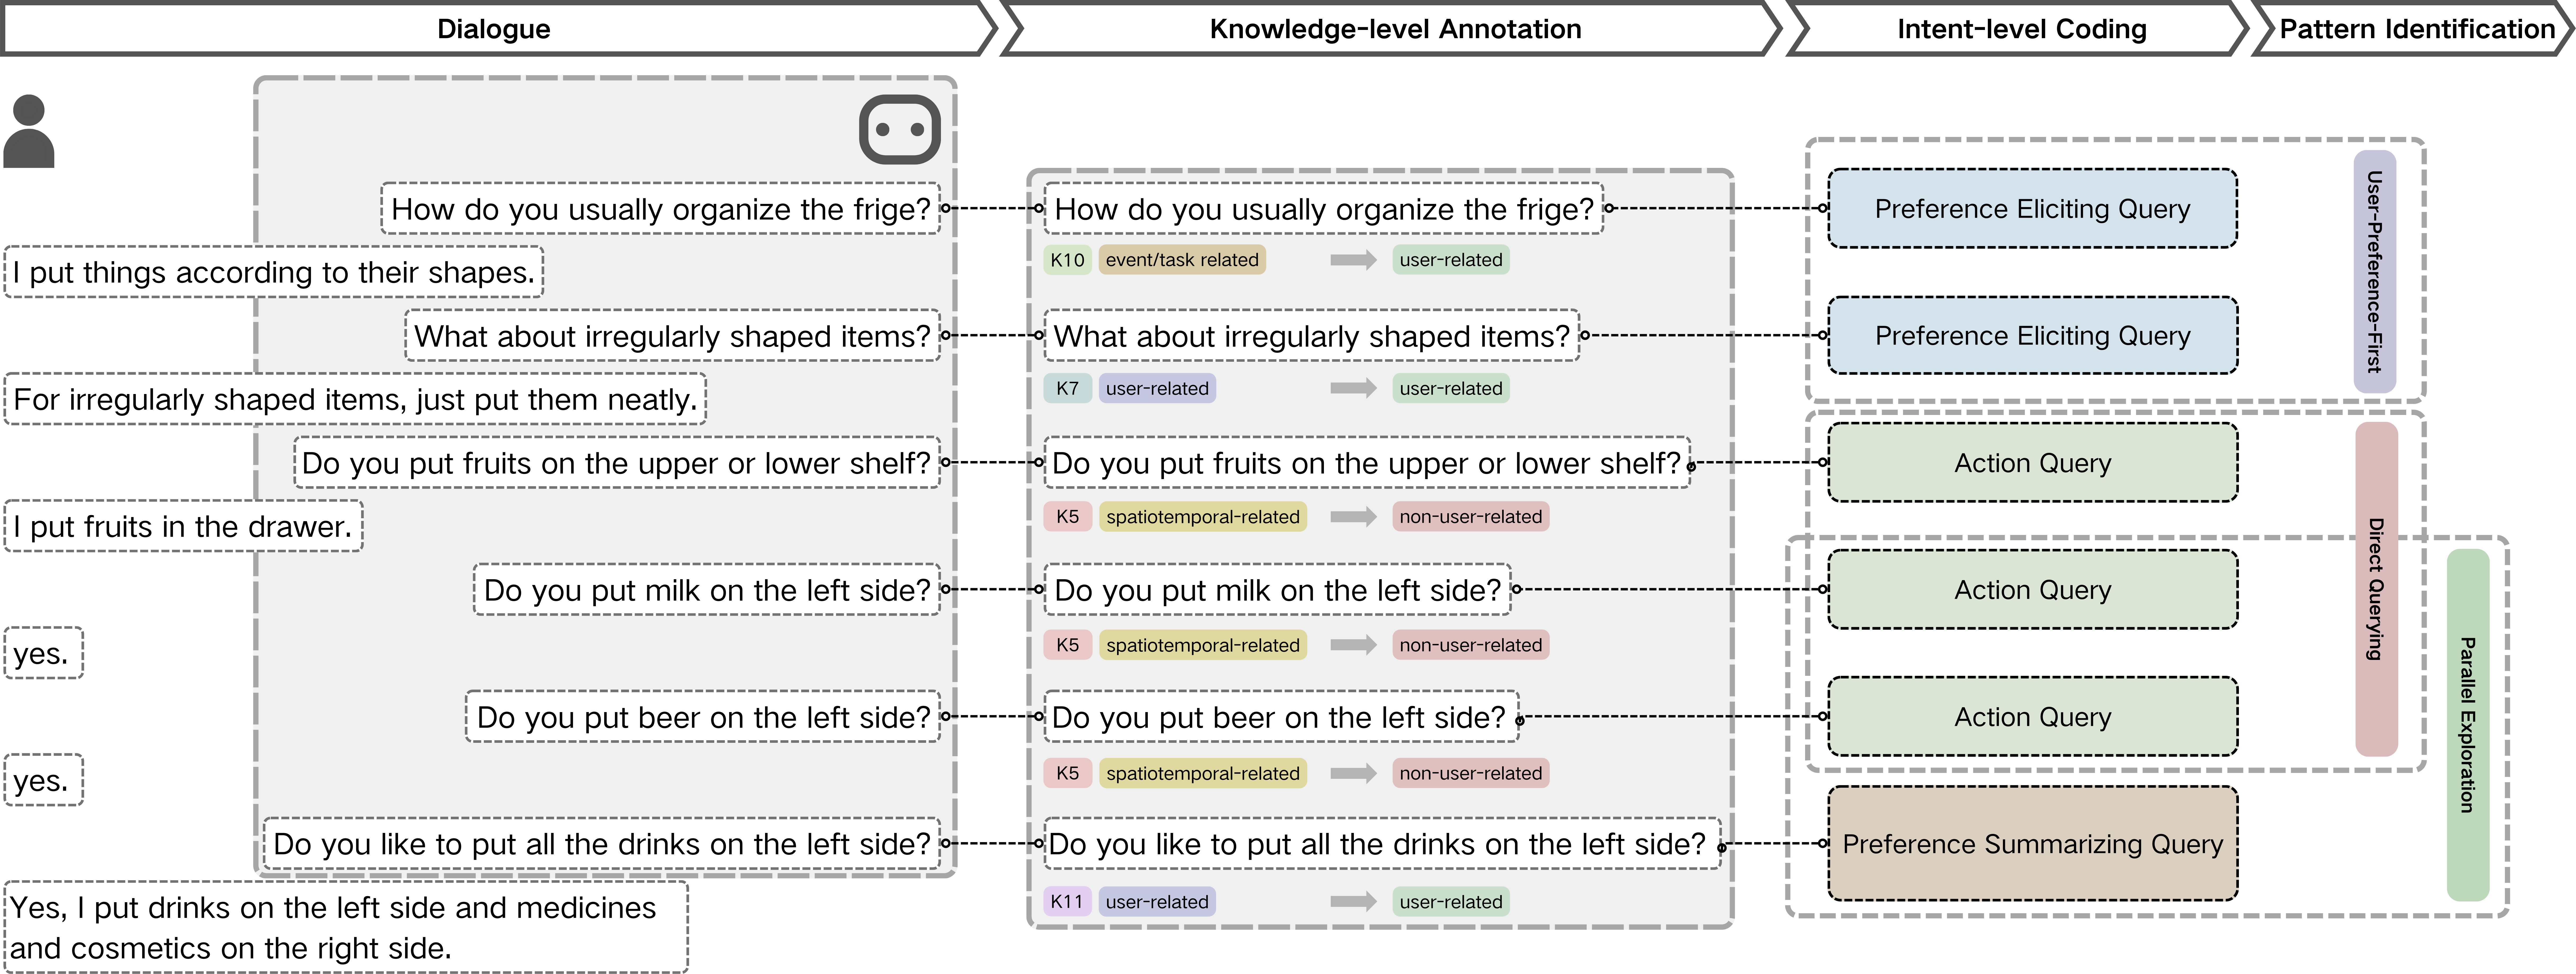
\includegraphics[width=\linewidth]{img/3.3.png}
  \caption{An illustration of the annotation pipeline: starting from raw human–robot dialogues, each question is first labeled by knowledge type, then coded for interactional intent, and finally abstracted into higher-level questioning patterns. This hierarchical process bridges low-level utterances and dialogue-level strategies.}
  \label{fig:annotation-pipeline}
\end{figure}

\subsubsection{Knowledge-level Annotation}
At the most fundamental level, we annotated each question with its corresponding knowledge type. To this end, we combined the K-type framework~\cite{shin2023uncertainty} with Wilson’s model of information behavior~\cite{wilson1999models}, allowing us to capture both the knowledge content of the question and whether it reflects user preferences. 

The K-type framework originates from cognitive psychology and educational research~\cite{redfield1981meta}~\cite{tofade2013best}, and enables a fine-grained categorization of questions according to the type of knowledge being solicited. It contains 11 categories ranging from objective factual knowledge (e.g., object identity, quantity, spatial location) to more complex subjective information (e.g., intentions, preferences, mental states). For example:
\begin{itemize}
    \item ``Is this a face mask?'' $\rightarrow$ Object Identity (K1);
    \item ``Should all the unopened stuff go on this shelf?'' $\rightarrow$ Spatial Layout (K5);
    \item ``Which part should we organize next?'' $\rightarrow$ Procedure (K8);
    \item ``Do you usually keep all the drinks on the door?'' $\rightarrow$ Internal State (K11).
\end{itemize}

We assume that the knowledge type of a question partly reflects the asker’s cognitive intent, as the focus of a question during task execution can indicate the asker’s immediate goals. The full K-type categories are presented in the Appendix (Table~\ref{tab:k-type}). 

However, while the K-type framework provides detailed knowledge classification, it does not explicitly account for task context or user preferences. For instance, the question ``Do you want the juice on the bottom or the top?'' would be classified as Spatial Layout (K5) under K-type, yet its core function is to \textit{elicit the user’s preference}, which K-type alone cannot capture. 

To address this limitation, we incorporated Wilson’s information behavior model as a complementary dimension. This model classifies questions according to information focus and task context, such as Object-related, Spatiotemporal-related, Event/Task-related, and User-related. In this study, we place particular emphasis on user preferences, and therefore we simplified the coding into two categories: \textbf{User-related}: Questions concerning user preferences, habits, or decisions; \textbf{Non-user-related}: Questions that do not involve user preferences.


In summary, each question was assigned two labels: (1) its knowledge type according to the K-type framework, and (2) whether it was user-related or non-user-related according to Wilson’s model. Figure~\ref{fig:annotation-pipeline} illustrates the distribution of several sample questions under this dual classification scheme. As shown, while multiple questions may share the same K-type category (e.g., Spatial Layout K5 or Procedure K8), Wilson’s complementary dimension allows us to further distinguish those that involve user preferences, thereby revealing the functional differences of questions within the interaction process more clearly.

\subsubsection{Intent-level Coding}
Annotating knowledge type alone is insufficient to reveal the actual function of a question in dialogue. Even when two questions share the same knowledge type, they may serve very different purposes in interaction. To capture these differences, we conducted a higher-level coding of each question based on its \textit{intent}, identifying what the asker aimed to achieve in a given context. 

Through iterative comparison and discussion, we distilled three stable categories of interactional intent, each with clear coding criteria:  \textbf{Action-oriented queries}. These questions focus on the concrete execution of the task and aim to clarify “how to do” something. If a question concerns the properties of an object, spatial arrangement, or procedural steps without involving user preferences, we coded it as action-oriented. For example, \textit{``Should this notebook be placed in the drawer?''} directly advances task execution. \textbf{Preference-summarizing queries}. As dialogues progress, questions often shift toward integrating and confirming previously gathered information. Such questions typically take a summarizing or hypothetical tone, inviting the user to confirm or correct. Questions beginning with phrases like \textit{``So\ldots''} or \textit{``Is it correct that\ldots''}
and drawing inferences from earlier answers were coded as preference-summarizing. For instance, \textit{``So you prefer to keep drinks on the upper shelf, right?''} represents this type. \textbf{Preference-eliciting queries}. These questions usually occur in the early or middle stages of a task and aim to gather the user’s overall tendencies or preferences at a choice point. The criterion here is whether the question explicitly prompts the user to select among multiple possible options. A typical example is \textit{``Do you want fruits placed above or below the drinks?''}. Such questions help the learner gradually build an understanding of the teacher’s habits.


By coding questions at the level of intent, we transform static knowledge annotations into dynamic representations of interactional goals, thereby uncovering the functional role of questions in task collaboration.


\subsubsection{Pattern Identification}
{\revstart
After completing intent-level coding for individual questions, we treated the entire dialogue sequence as the unit of analysis to identify recurring questioning patterns. For each dialogue, we constructed an \textit{intent sequence}---the ordered list of intent codes (AO, PE, PS) across all questions---and analyzed the temporal distribution and transition structure of different intent types. Specifically, we examined: (1)~which intent types appeared in the opening, middle, and closing segments of each dialogue; (2)~whether preference-related intents (PE, PS) clustered at the beginning, were distributed throughout, or were absent entirely; and (3)~the dominant transition patterns between consecutive intent types.

Two researchers independently classified each of the 28 dialogue sequences into candidate patterns using the criteria below, achieving an inter-rater agreement of $\kappa = $~\textbf{TODO} at the pattern level. Disagreements were resolved through discussion. This process yielded three stable and representative questioning patterns.
\revend}
% TODO: Fill in actual Cohen's kappa for pattern-level agreement.

\begin{itemize}
    \item \textbf{User-Preference-First}. In this pattern, participants typically begin the dialogue by directly asking about the user’s personal habits or preferences, which then serve as the basis for subsequent decisions. The criterion is that if the first question in the sequence is classified as a preference-eliciting query and is followed mainly by action-oriented queries, the sequence is coded as User-Preference-First. This reflects a \textit{top-down} reasoning pathway: establishing global high-level rules first, then mapping them onto concrete operations. For example, the learner may begin with \textit{“Do you prefer to keep drinks on the door or inside the fridge?”} before proceeding with action-oriented questions such as \textit{“Should this milk be placed on the upper shelf?”}.
    
    \item \textbf{Parallel Exploration}. In this pattern, participants interleave action-oriented questions with preference-related ones throughout the task, thereby continuously integrating user preferences while advancing operations. The criterion is that preference-eliciting or preference-summarizing questions appear not only at the beginning but also in the middle or later stages of the sequence. This reflects a \textit{bottom-up} reasoning pathway: accumulating evidence through action-oriented queries and gradually extracting or validating high-level preferences, resulting in a “do-and-induce” loop. For example, while placing items, the learner may intermittently ask \textit{“Does this arrangement match your usual habit?”}.
    
    \item \textbf{Direct Querying}. Unlike the other two patterns, this type of dialogue is entirely focused on action-oriented questions, with little or no attempt to elicit or summarize user preferences. The criterion is that the entire sequence consists solely of action-oriented queries, without preference-eliciting or preference-summarizing ones. This reflects a single-layer, reactive logic in which the learner behaves more like an executor of instructions than an interpreter of user preferences.
\end{itemize}

In summary, these three patterns reveal different organizational logics of multi-turn questioning: User-Preference-First emphasizes top-down reasoning, Parallel Exploration emphasizes iterative alternation between low- and high-level reasoning, while Direct Querying remains at the level of immediate operations, as shown in 
Figure~\ref{fig:annotation-framework}.

\begin{figure}[t]
  \centering
  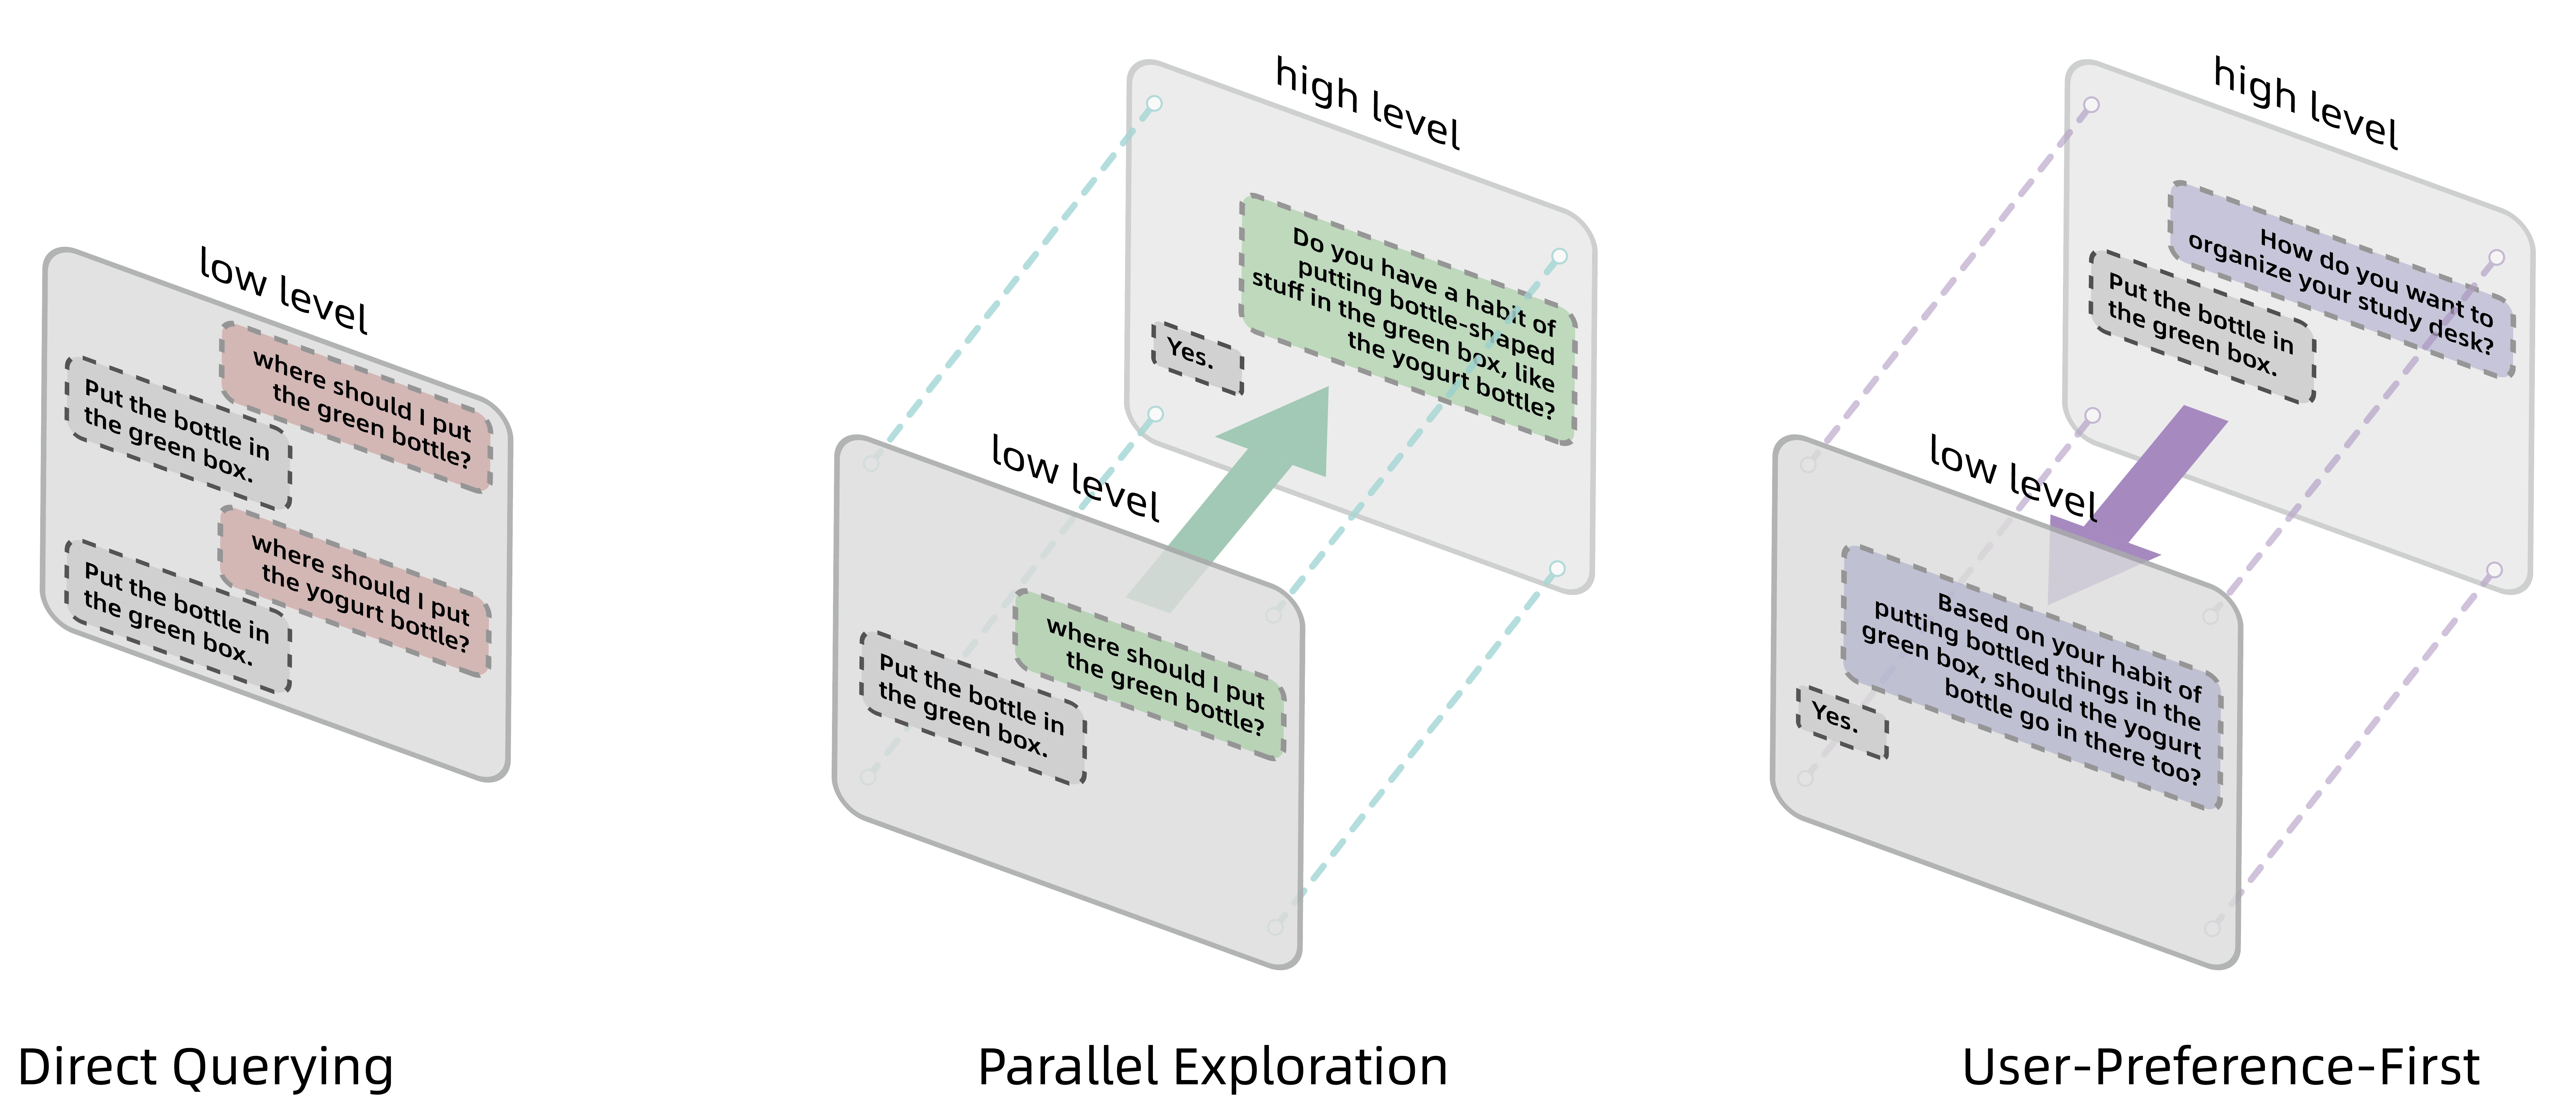
\includegraphics[width=\linewidth]{img/3.3.3.png}
  \caption{Hierarchical coding framework for analyzing questioning strategies. 
  The process begins with knowledge-level annotation, proceeds to intent-level coding, and culminates in the identification of higher-level conversational patterns and strategies.}
  \label{fig:annotation-framework}
\end{figure}


\subsection{Pattern Distribution}
Although some dialogues exhibited within-sequence shifts between questioning patterns, for comparability we adopted a \textit{dominant-pattern} labeling: each dialogue was assigned to the single pattern that best captured its overall trajectory. This choice prioritizes analytical clarity at the dialogue level and enables robust between-task comparisons.

Based on this labeling, we compared distributions across tasks. In the 14 \textit{refrigerator organization} dialogues, 9 sequences (64.3\%) followed \textit{User-Preference-First}, 3 (21.4\%) exhibited \textit{Parallel Exploration}, and 2 (14.3\%) were \textit{Direct Querying}. In contrast, among the 14 \textit{cocktail mixing} dialogues, 2 sequences (14.3\%) adopted \textit{User-Preference-First}, 10 (71.4\%) followed \textit{Parallel Exploration}, and 2 (14.3\%) were \textit{Direct Querying}.

\rev{A Fisher's exact test confirmed that the distribution of dominant patterns differed significantly between the two tasks ($p = $~\textbf{TODO}), indicating that task structure influences which questioning pattern participants adopt. The refrigerator task---which centers on achieving a desired \textit{final state}---favored the top-down User-Preference-First pattern, while the cocktail task---which emphasizes \textit{procedural steps}---favored the iterative Parallel Exploration pattern. Direct Querying appeared at a low but consistent rate (14.3\%) in both tasks. These results confirm that all three patterns are empirically grounded and that their relative prevalence is modulated by task characteristics.}
% TODO: Fill in Fisher's exact test p-value from the 3x2 contingency table.


\section{System Design}
\label{sec:system-design}
{\revstart

\subsection{From Questioning Patterns to Questioning Strategies}

Our HHI study (Section~3) revealed that people organize questions at three distinct levels of abstraction: Action-Oriented (AO) queries that resolve individual placements, Preference-Eliciting (PE) queries that probe for general organizing rules, and Preference-Summarizing (PS) queries that consolidate previously gathered information. We treat these as \textit{questioning design patterns}---reusable interaction building blocks that capture recurring solutions to the problem of acquiring user preferences through dialogue.

Translating these design patterns into a computational system requires two steps. First, we formalize them as composable modules (Section~\ref{sec:question-patterns}). In this step, we refine PS into \textit{Preference-Induction} (PI): whereas PS in HHI passively restates information the learner already heard, PI actively proposes a testable hypothesis inferred from accumulated evidence and asks the user to confirm, refine, or reject it---a more effective mechanism for robotic dialogue where implicit inference is unavailable. The resulting three design patterns---AO, PE, and PI---serve as the atomic building blocks of our framework (Table~\ref{tab:patterns}).

Second, we compose these patterns into four \textit{questioning strategies} (Section~\ref{sec:strategies}) that define which patterns are available and how they are scheduled across the question budget (Table~\ref{tab:strategies}). Three strategies directly correspond to the dialogue-level behaviors observed in HHI (DQ~$\leftrightarrow$~Direct Querying, UPF~$\leftrightarrow$~User-Preference-First, PAR~$\leftrightarrow$~Parallel Exploration); a fourth---Hybrid-All (HYB)---adaptively selects among all patterns, serving as an upper-bound reference.

A key design decision is the use of a \textit{structured preference state} rather than retaining only raw dialogue history. While an end-to-end LLM could in principle read the entire conversation and produce placements, structured intermediate representations improve consistency and controllability in multi-turn reasoning~\cite{tyshka2023interactive}. Our structured state explicitly separates confirmed object placements, category-level organizing rules, and negative evidence, enabling the final placement planner to apply evidence hierarchically. We empirically validate this choice through a \textit{Raw LLM} baseline that operates on unstructured dialogue history alone (Section~\ref{sec:baselines}).


\subsection{Task Formulation}
\label{sec:task-formulation}

We consider a household rearrangement scenario defined by a tuple $(R, \mathcal{C}, \mathcal{O}_s, \mathcal{O}_u)$, where $R$ is the room type, $\mathcal{C} = \{c_1, \dots, c_M\}$ is the set of available receptacles (shelves, drawers, cabinets, etc.), and $\mathcal{O}_s$, $\mathcal{O}_u$ are the sets of \textit{seen} and \textit{unseen} objects, respectively. Seen objects are visible during the interaction; unseen objects must be placed based on preferences generalized from the dialogue. The agent may ask at most $B$ questions (the \emph{question budget}) before placing all objects.

This seen/unseen split provides a principled measure of generalization: a strategy that extracts transferable category-level rules should outperform one that only resolves individual placements on unseen objects, even when the two strategies perform similarly on seen objects.


\subsection{Structured Preference State}
\label{sec:structured-state}

Rather than retaining only raw dialogue history, the agent maintains a structured state $\mathcal{S}_t$ that separates different types of learned preference information:

\begin{itemize}[leftmargin=*]
    \item \textbf{Confirmed actions} $\mathcal{A}^+ = \{(o_i, c_j)\}$: specific object--receptacle pairs confirmed by the user (e.g., \textit{``the reading light goes on the nightstand’’}).
    \item \textbf{Confirmed preferences} $\mathcal{P}^+ = \{(h_k, O_k, c_k)\}$: category-level organizing rules, each consisting of a natural-language hypothesis $h_k$ describing the category (e.g., \textit{``fragile glass and ceramic drinkware’’}), a set of covered objects $O_k \subseteq \mathcal{O}_s$, and optionally a target receptacle $c_k$.
    \item \textbf{Negative actions} $\mathcal{A}^-$: object--receptacle pairs explicitly rejected.
    \item \textbf{Negative preferences} $\mathcal{P}^-$: category-level hypotheses rejected by the user.
    \item \textbf{Unresolved objects} $\mathcal{U}_t = \mathcal{O}_s \setminus \{o : (o, \cdot) \in \mathcal{A}^+\}$: seen objects not yet assigned to a receptacle.
\end{itemize}

This structured representation serves two purposes. First, it enables the \textit{strategy controller} to reason about what information is still missing (e.g., which receptacles lack any confirmed preference) and select the most informative questioning pattern accordingly. Second, it provides the \textit{final placement planner} with hierarchical evidence for placement inference: confirmed preferences take priority over action-based analogy, which in turn takes priority over general commonsense.


\subsection{Three Questioning Design Patterns}
\label{sec:question-patterns}

We formalize the three intent categories from our HHI study as three \textit{questioning design patterns}, each implemented as an independent LLM-based proposer module:

\subsubsection{Action-Oriented (AO)}
AO questions directly ask about the placement of a single specific object (e.g., \textit{``Where should the reading light go?’’}). Each AO question resolves one object’s placement, yielding a confirmed action $(o_i, c_j)$. This corresponds to the \textit{Direct Querying} pattern observed in HHI, where learners proceed item-by-item without attempting to elicit broader rules.

The AO proposer selects a target object from the unresolved set $\mathcal{U}_t$, prioritizing objects that belong to receptacles not yet covered by any confirmed preference or action, and avoiding repetition with recent questions.

\subsubsection{Preference-Eliciting (PE)}
PE questions ask about the user’s organizing \textit{habits or principles} for a category of objects (e.g., \textit{``How do you usually organize electronic accessories---do they tend to stay in one spot?’’}). A successful PE exchange yields a confirmed preference $(h_k, O_k, c_k)$ that can generalize to multiple seen and unseen objects simultaneously.

The PE proposer first builds candidate hypotheses by grouping unresolved objects into potential categories based on shared attributes (material, size, usage context). It then selects the most informative candidate---prioritizing categories that cover uncovered receptacles---and generates a natural-language question. This corresponds to the \textit{User-Preference-First} pattern, where learners establish general rules before addressing specific items.

\subsubsection{Preference-Induction (PI)}
PI questions propose a rule \textit{inferred from previously confirmed actions} and ask the user to confirm, refine, or reject it (e.g., \textit{``I noticed you placed the remote and speaker both in the media drawer---do you generally keep handheld electronics there?’’}). Unlike PE, which probes for rules top-down, PI works bottom-up: it consolidates accumulated evidence into a testable hypothesis.

The PI proposer examines confirmed actions $\mathcal{A}^+$ to find receptacles with multiple confirmed objects, then generates a category-level hypothesis that explains these placements. This corresponds to the \textit{Parallel Exploration} pattern, where learners interleave concrete actions with periodic induction of broader rules.

Table~\ref{tab:patterns} summarizes the three questioning patterns with their descriptions and examples.

\begin{table}[t]
\centering
\caption{\rev{Three questioning design patterns extracted from HHI and formalized for robotic dialogue. Each pattern targets a different level of preference information. PS (Preference-Summarizing), observed in HHI, is operationalized as PI (Preference-Induction) in our system.}}
\label{tab:patterns}
\begin{tabularx}{\linewidth}{@{} l >{\raggedright\arraybackslash}X >{\raggedright\arraybackslash}X @{}}
\toprule
\textbf{Pattern} & \textbf{Description} & \textbf{Example} \\
\midrule
\rev{\textbf{Action-Oriented (AO)}} &
\rev{Asks about the placement of one specific object. Yields a confirmed action $(o_i, c_j)$.} &
\rev{``Where should the reading light go?''} \\
\midrule
\rev{\textbf{Preference-Eliciting (PE)}} &
\rev{Asks about the user's organizing habit or principle for a \textit{category} of objects. Yields a confirmed preference $(h_k, O_k, c_k)$ that generalizes to multiple objects.} &
\rev{``How do you usually organize electronic accessories---do they tend to stay in one spot?''} \\
\midrule
\rev{\textbf{Preference-Induction (PI)}} &
\rev{Proposes a rule \textit{inferred from confirmed actions} and asks the user to confirm, refine, or reject it. Yields a confirmed or rejected preference.} &
\rev{``I noticed the remote and speaker both went to the media drawer---do you keep handheld electronics there in general?''} \\
\bottomrule
\end{tabularx}
\end{table}


\subsection{Questioning Strategies}
\label{sec:strategies}

A \textit{questioning strategy} determines which questioning patterns are available and in what order they are deployed across the budget. We define four strategies that systematically vary the composition and scheduling of AO, PE, and PI (Table~\ref{tab:strategies}):

\begin{table*}[t]
\centering
\caption{\rev{Four questioning strategies, their questioning pattern composition, and example dialogue sequences generated by the system. The first three correspond to HHI patterns (Section~3); HYB is an adaptive combination. AO = Action-Oriented, PE = Preference-Eliciting, PI = Preference-Induction.}}
\label{tab:strategies}
\begin{tabularx}{\textwidth}{@{} l c >{\raggedright\arraybackslash}p{4.2cm} >{\raggedright\arraybackslash}X @{}}
\toprule
\textbf{Strategy} & \textbf{Types} & \textbf{Scheduling Logic} & \textbf{Example Dialogue (budget=4)} \\
\midrule
DQ & AO & One AO per turn. No preference elicitation or induction. &
\rev{Q1: ``Where should the reading light go?'' (AO) $\to$ Q2: ``Where does the novel go?'' (AO) $\to$ Q3: ``Where should the remote go?'' (AO) $\to$ Q4: ``Where does the speaker go?'' (AO)} \\
\midrule
UPF & PE $\to$ AO & Begin with PE for uncovered receptacles; switch to AO boundary probing once all receptacles have $\geq$1 confirmed preference. &
\rev{Q1: ``How do you organize electronic accessories?'' (PE) $\to$ Q2: ``What about reading materials?'' (PE) $\to$ Q3: ``Where should the desk lamp go?'' (AO, boundary) $\to$ Q4: ``Does the puzzle book go with reading or games?'' (AO, boundary)} \\
\midrule
PAR & AO $\to$ PI & Begin with AO; after 2+ actions on a receptacle, trigger PI to consolidate evidence into a rule. &
\rev{Q1: ``Where should the remote go?'' (AO) $\to$ Q2: ``Where does the speaker go?'' (AO) $\to$ Q3: ``Both went to the media drawer---do handheld electronics all go there?'' (PI) $\to$ Q4: ``Where should the desk lamp go?'' (AO)} \\
\midrule
HYB & PE+AO+PI & Adaptive: PE when gaps remain; AO when last PE was weak; PI when unsummarized actions accumulate. &
\rev{Q1: ``How do you organize items on the bookshelf?'' (PE) $\to$ Q2: ``Where should the remote go?'' (AO, PE was weak) $\to$ Q3: ``Where does the speaker go?'' (AO) $\to$ Q4: ``Both went to the media drawer---electronics there?'' (PI)} \\
\bottomrule
\end{tabularx}
\end{table*}

\paragraph{Direct Querying (DQ).} DQ uses only AO questions throughout the entire budget. Each question resolves one object’s placement, yielding $B$ confirmed actions after $B$ questions. DQ serves as a strong baseline: it makes no attempt to learn generalizable rules, but it accumulates maximal concrete evidence for the placement planner’s semantic analogy step.

\paragraph{User-Preference-First (UPF).} UPF begins with PE questions to discover category-level organizing rules, prioritizing receptacles that lack any confirmed preference or action. Once all receptacles have at least one confirmed rule, the strategy switches to AO questions that probe \textit{boundary cases}---objects whose category membership is ambiguous given the current rules. This top-down approach mirrors the human pattern of establishing global principles before addressing specific items.

\paragraph{Parallel Exploration (PAR).} PAR begins with AO questions to collect concrete placement evidence. After two or more consecutive AO turns, if a receptacle has accumulated multiple confirmed actions without a corresponding confirmed preference, the strategy triggers a PI question to consolidate that evidence into a rule. This bottom-up approach mirrors the human pattern of interleaving actions with periodic induction.

\paragraph{Hybrid-All (HYB).} HYB has access to all three questioning patterns and selects adaptively. After each PE question, the system evaluates whether the resulting preference is ``strong’’ (covers $\geq$2 objects and resolves to a specific receptacle). If the preference is weak, the system falls back to AO to collect concrete evidence. When unsummarized confirmed actions accumulate ($\geq$2 actions on a receptacle without a corresponding rule), the system triggers PI for consolidation.

The scheduling logic is implemented as deterministic, rule-based heuristics in the strategy controller, ensuring reproducibility across experiments. An entropy-driven selection method based on Expected Entropy Reduction (EER) is also available as an alternative.


\subsection{State Update}
\label{sec:state-update}

After each question--answer exchange, the \textit{State Update} module interprets the user’s natural-language answer and updates the structured state $\mathcal{S}_t$. The interpretation follows one of three paths, determined by the question pattern:

\begin{itemize}[leftmargin=*]
    \item \textbf{AO answer interpretation:} The LLM classifies the answer as a \textit{direct placement} (yields a confirmed action), an \textit{exclusion} (yields a negative action), or a \textit{general rule} (yields a confirmed preference discovered incidentally).
    \item \textbf{PE answer interpretation:} The LLM extracts a \textit{category-level rule} from the answer, identifies which objects are covered by the rule, and determines whether the user rejected the proposed hypothesis. If accepted, the rule is added to $\mathcal{P}^+$; if rejected, it is recorded in $\mathcal{P}^-$.
    \item \textbf{PI answer interpretation:} The LLM determines whether the user \textit{confirmed}, \textit{refined}, or \textit{rejected} the proposed hypothesis. Confirmed or refined hypotheses are added to $\mathcal{P}^+$; rejected hypotheses are recorded in $\mathcal{P}^-$. A special \textit{rule-with-exception} case handles partial confirmation where one object deviates from the general rule.
\end{itemize}

After each update, the set of unresolved objects $\mathcal{U}_t$ is recomputed by removing objects that appear in confirmed actions. All interpretations are generated by a single LLM call with pattern-specific system prompts that enforce structured output, and the results are validated against the current state to prevent contradictions.


\subsection{Final Placement Planner}
\label{sec:final-planner}

After the question budget is exhausted, the \textit{Final Placement Planner} assigns receptacles to all remaining objects in two stages:

\paragraph{Seen object placement.} For each unresolved seen object $o \in \mathcal{U}_B$, the planner applies evidence in priority order: (1)~confirmed preferences---if $o$ fits a preference category, assign it to that preference’s receptacle; (2)~confirmed action analogy---find the most semantically similar confirmed object by function and usage context, and apply the same receptacle; (3)~general reasoning fallback. Negative actions $\mathcal{A}^-$ are respected as hard constraints throughout.

\paragraph{Unseen object placement.} For each unseen object $o \in \mathcal{O}_u$, the planner follows the same priority but with emphasis on attribute-based matching: material, size, power source, and usage context determine which confirmed preference best fits the unseen object. When multiple preferences could match, the planner uses distinguishing attributes (e.g., \textit{small} vs. \textit{large}, \textit{for play} vs. \textit{for reading}) to select the most specific match.

This two-stage design ensures that confirmed evidence always overrides general commonsense knowledge, which is critical for personalized household tasks where user preferences may diverge from common organizational norms.


\subsection{Baselines}
\label{sec:baselines}

To isolate the contribution of the structured questioning framework, we introduce two baselines:

\paragraph{No Question.} The agent receives the task specification (room, receptacles, objects) but asks zero questions ($B=0$). The Final Placement Planner operates on the initial state with empty evidence, relying entirely on the LLM’s commonsense knowledge. This baseline establishes the lower bound of what can be achieved without any user interaction.

\paragraph{Raw LLM.} The agent asks up to $B$ questions using an unconstrained LLM---without any questioning strategy, structured state representation, or pattern-specific proposers. Questions are generated freely based on the task context and conversation history. After the budget is exhausted, a separate LLM reads the raw conversation history and produces placement decisions directly, without structured intermediate state. This baseline isolates the contribution of the entire strategy framework (strategy scheduling + structured state + evidence-based planner) by comparing it against a pure end-to-end LLM approach.

% TODO: Add new system architecture figure to replace old QUEST diagram
% \begin{figure*}[t]
%   \centering
%   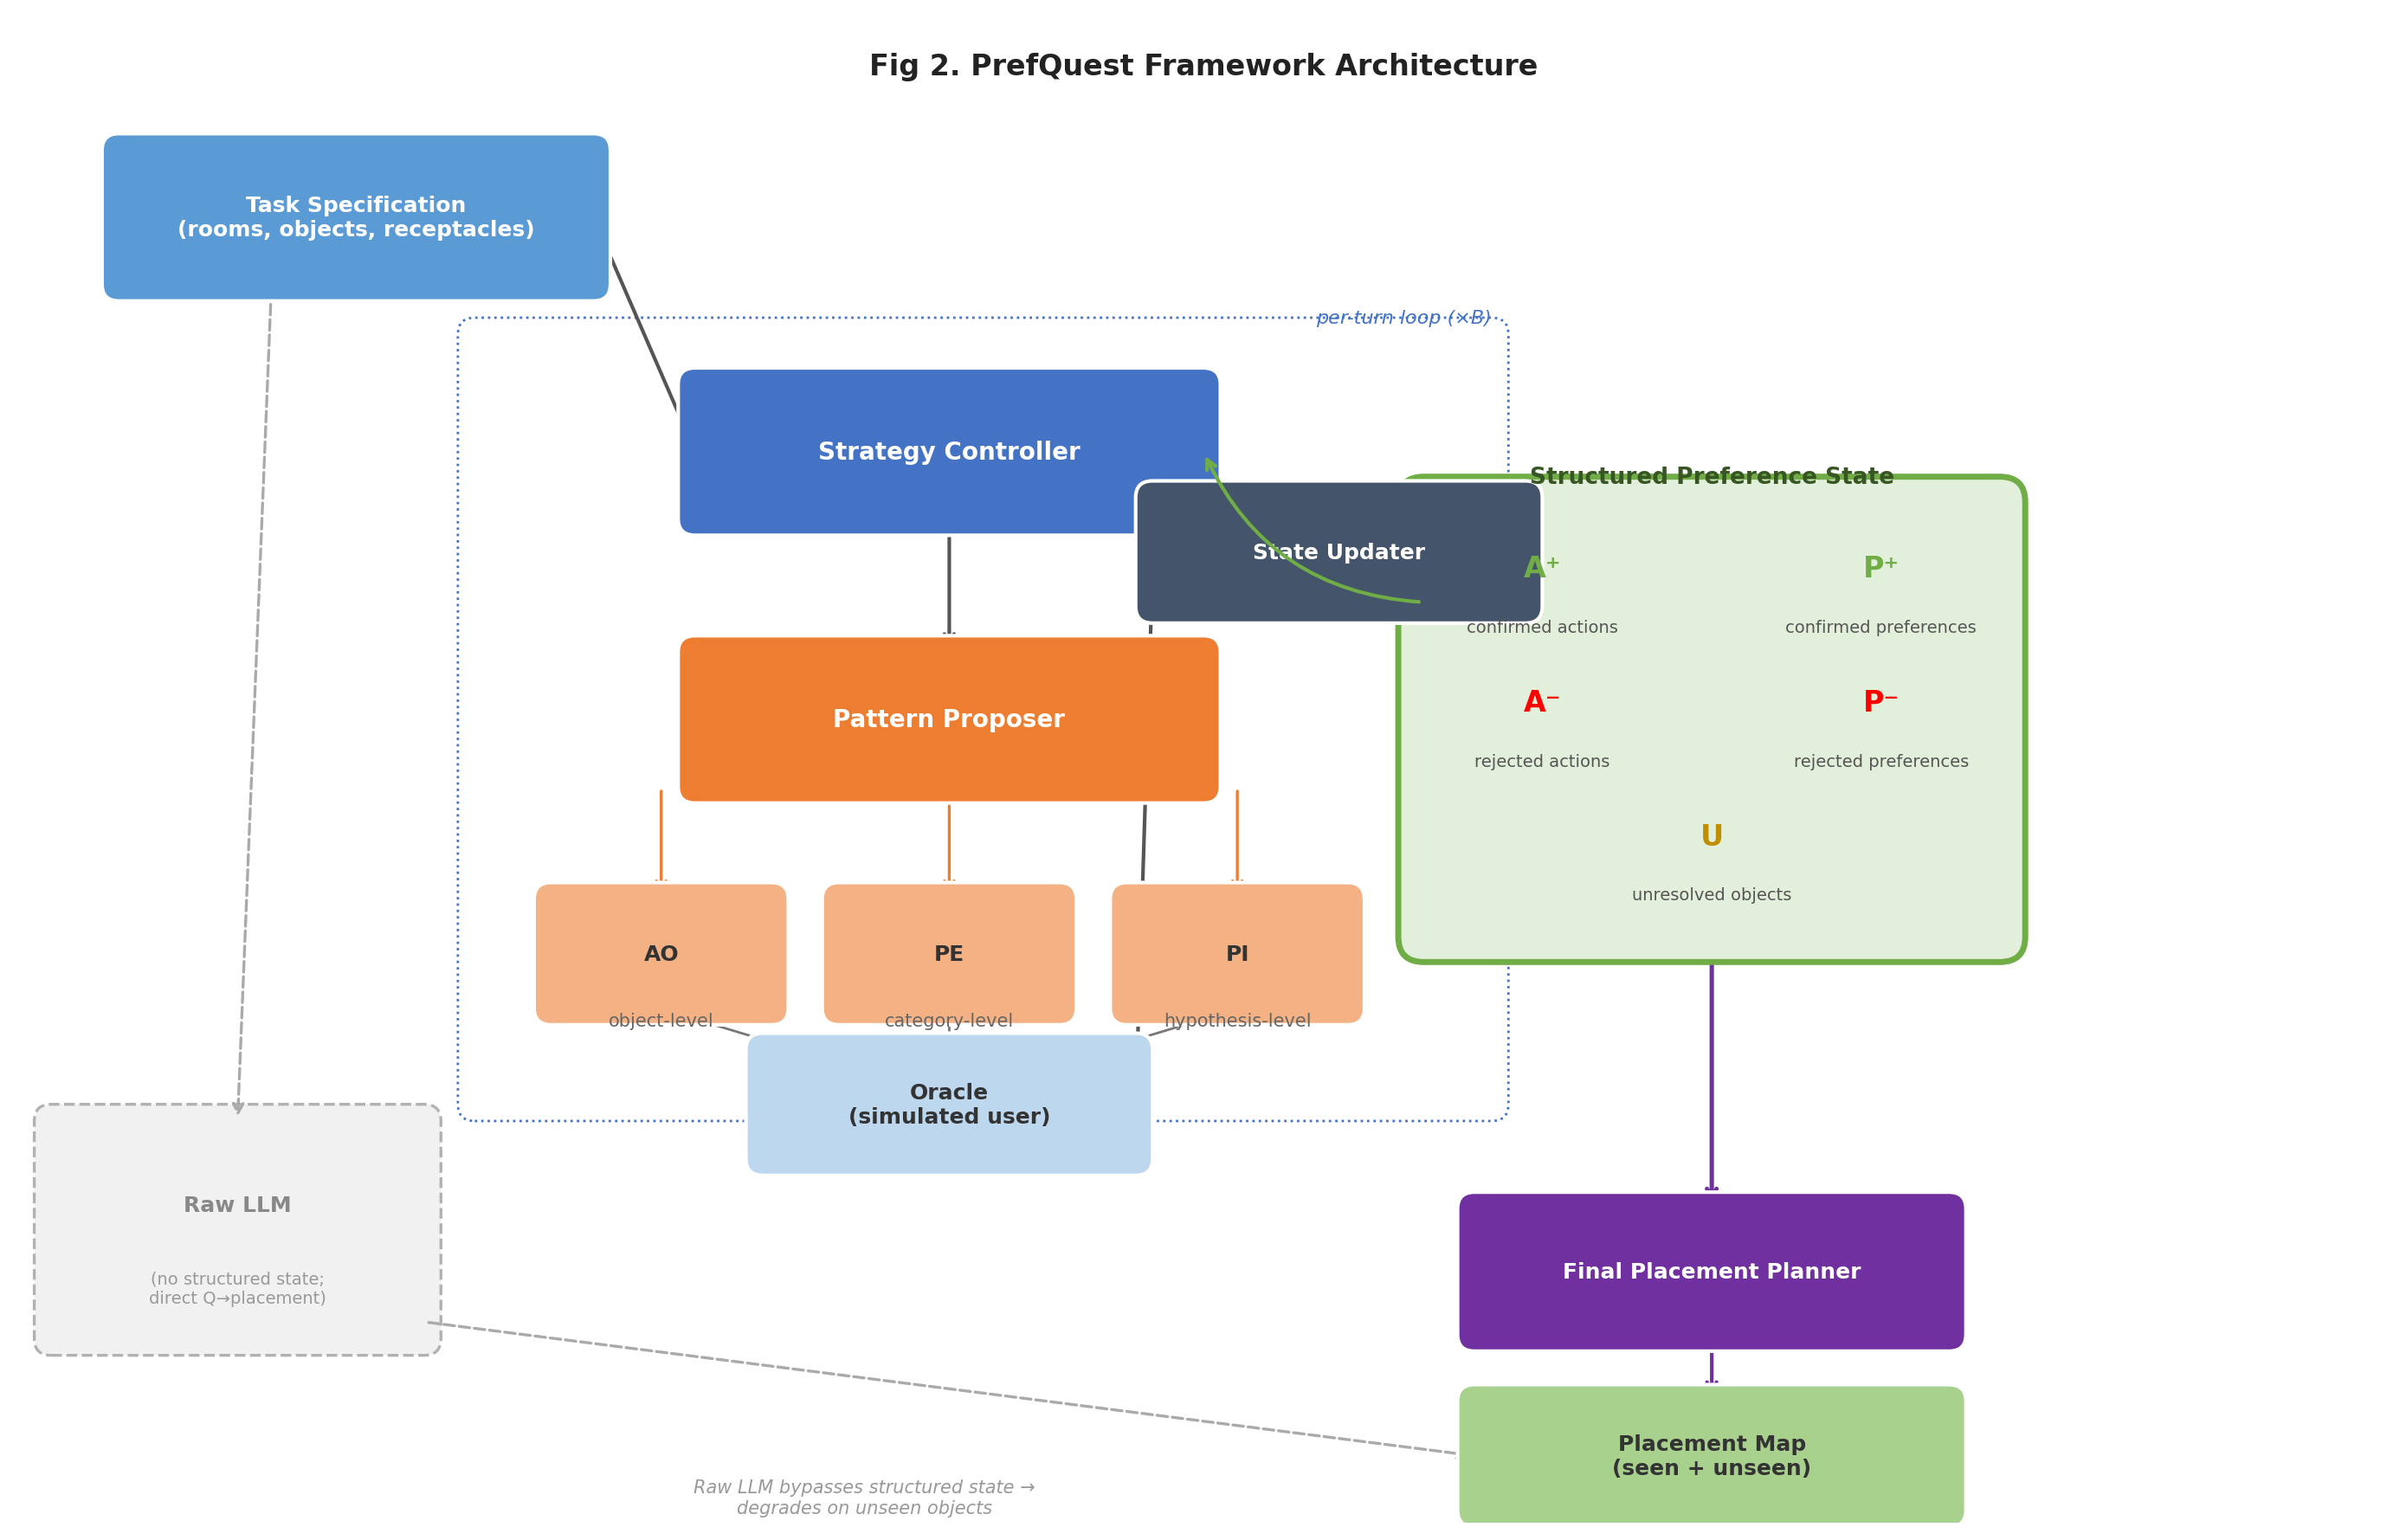
\includegraphics[width=\textwidth]{img/system-v2.png}
%   \caption{Overview of the revised system architecture. The dialogue loop consists of: (1) the Policy Controller selects a question pattern based on the current structured state and strategy; (2) a pattern-specific Proposer generates the question; (3) the user (or simulated Oracle) answers; (4) the State Update module extracts structured evidence from the answer; (5) after the budget is exhausted, the Final Placement Planner assigns all remaining objects using the accumulated evidence.}
%   \label{fig:system-architecture}
% \end{figure*}
\revend}

\section{Study 1: Characterizing Strategy Performance Through Simulation}
\label{sec:study1}
{\revstart

Study~1 aims to establish controlled performance baselines for each strategy and to characterize how their accuracy profiles differ across question budgets. By using LLM-simulated users (oracles), we can run experiments at a scale that would be infeasible with human participants, enabling systematic comparison across 102 household episodes and multiple budget values.

\subsection{Dataset}

We constructed a dataset of 102 household episodes spanning three room types: living rooms (34 episodes), bedrooms (34 episodes), and kitchens (34 episodes). Each episode contains 12 seen objects, 15--22 unseen objects (mean~19.1), and 5 receptacles. The asymmetric split---more unseen than seen---provides a rigorous test of generalization: strategies must extrapolate from limited evidence to a larger set of novel objects.

Each episode includes annotator-authored natural-language notes describing the user’s organizing principles (e.g., \textit{``Handheld media-control and portable entertainment devices go to the media drawer’’}). These notes serve as ground truth for the simulated oracle’s responses but are never directly revealed to the agent. Critically, every receptacle has at least one seen object assigned to it, ensuring that all strategies have a fair opportunity to discover evidence for every receptacle through their respective questioning patterns.

\subsection{Oracle Design}

We employ an LLM-based \textit{Natural User Oracle} that simulates a cooperative household member. Given a question, the oracle generates a natural-language answer grounded in the episode’s annotator notes and ground-truth placements. Unlike a simple lookup table, the oracle produces varied, realistic responses that may include partial information, category-level rules, or exceptions---mirroring the complexity of real human answers.

The oracle is constrained to: (1)~never directly quote or paraphrase the annotator notes; (2)~use exact receptacle names from the provided list; (3)~maintain consistency with previous answers in the dialogue history; and (4)~honestly state when no specific organizing rule applies.

\subsection{Experimental Setup}

\paragraph{Conditions.} We evaluate six conditions: four questioning strategies (DQ, UPF, PAR, HYB) and two baselines (No Question, Raw LLM). All conditions use the same dataset, oracle, and evaluation procedure.

\paragraph{Budget.} Each strategy is evaluated at budget checkpoints $B \in \{1, 2, \dots, 10\}$. For efficiency, each episode is run once up to $B_{\max}=10$, with the structured state evaluated at each checkpoint. The No Question baseline corresponds to $B=0$.

\paragraph{Models.} The primary model is Qwen3-8B served via Ollama (102 episodes, all conditions). For cross-model validation, we additionally run experiments with GPT-5-Chat via the OpenAI-compatible API.
% TODO: Add gpt-5-chat full results when available.

\paragraph{Metrics.} For each episode and budget, we compute:
\begin{itemize}[leftmargin=*]
    \item \textbf{Seen accuracy}: fraction of seen objects assigned to their ground-truth receptacle.
    \item \textbf{Unseen accuracy}: fraction of unseen objects assigned to their ground-truth receptacle.
\end{itemize}
We report mean accuracy $\pm$ standard error across 102 episodes. Unseen accuracy is the primary metric of interest, as it directly measures the agent’s ability to generalize learned preferences to novel objects.

\subsection{Hypotheses}

\begin{itemize}[leftmargin=*]
    \item \textbf{H1}: All strategies improve seen accuracy monotonically with budget.
    \item \textbf{H2}: PE-based strategies (UPF, HYB) achieve significantly higher unseen accuracy than AO-only (DQ) at moderate budgets ($B \geq 3$), because category-level rules generalize to unseen objects.
    \item \textbf{H3}: PI-based strategy (PAR) does not significantly outperform DQ on unseen accuracy, because bottom-up induction requires multiple AO turns before a rule can be proposed, reducing budget efficiency.
    \item \textbf{H4}: HYB does not significantly outperform UPF, indicating that adaptive pattern selection provides no advantage over the simpler PE-first heuristic.
    \item \textbf{H5}: All strategies significantly outperform the No Question baseline on both metrics.
    \item \textbf{H6}: Strategy-based approaches outperform Raw LLM on unseen accuracy, validating the value of structured preference state over end-to-end LLM reasoning.
\end{itemize}

\subsection{Results}

\subsubsection{Overall Performance}

Table~\ref{tab:study1-results} presents the main results at selected budget checkpoints. Figure~\ref{fig:ablation-curves} shows the full accuracy curves across all budgets.

\begin{table*}[t]
\centering
\caption{Seen and unseen accuracy (mean $\pm$ SE) across 102 episodes for each condition at selected budgets. Model: Qwen3-8B.}
\label{tab:study1-results}
\begin{tabular}{l cc cc cc cc}
\toprule
 & \multicolumn{2}{c}{$B=0$} & \multicolumn{2}{c}{$B=3$} & \multicolumn{2}{c}{$B=5$} & \multicolumn{2}{c}{$B=10$} \\
\cmidrule(lr){2-3} \cmidrule(lr){4-5} \cmidrule(lr){6-7} \cmidrule(lr){8-9}
\textbf{Condition} & Seen & Unseen & Seen & Unseen & Seen & Unseen & Seen & Unseen \\
\midrule
No Question & .501 & .507 & --- & --- & --- & --- & --- & --- \\
% TODO: Raw LLM results pending
Raw LLM & --- & --- & --- & --- & --- & --- & --- & --- \\
\midrule
DQ  & --- & --- & .667{\scriptsize$\pm$.015} & .553{\scriptsize$\pm$.014} & .753{\scriptsize$\pm$.012} & .587{\scriptsize$\pm$.014} & .931{\scriptsize$\pm$.006} & .631{\scriptsize$\pm$.013} \\
UPF & --- & --- & .616{\scriptsize$\pm$.016} & .560{\scriptsize$\pm$.013} & .792{\scriptsize$\pm$.017} & \textbf{.698}{\scriptsize$\pm$.014} & .874{\scriptsize$\pm$.016} & \textbf{.715}{\scriptsize$\pm$.013} \\
PAR & --- & --- & .650{\scriptsize$\pm$.015} & .548{\scriptsize$\pm$.015} & .721{\scriptsize$\pm$.013} & .572{\scriptsize$\pm$.015} & .858{\scriptsize$\pm$.009} & .615{\scriptsize$\pm$.014} \\
HYB & --- & --- & .620{\scriptsize$\pm$.018} & .574{\scriptsize$\pm$.014} & .771{\scriptsize$\pm$.019} & .682{\scriptsize$\pm$.016} & .835{\scriptsize$\pm$.018} & .695{\scriptsize$\pm$.015} \\
\bottomrule
\end{tabular}
\end{table*}

% TODO: Replace with final version including Raw LLM + gpt-5-chat
\begin{figure*}[t]
  \centering
  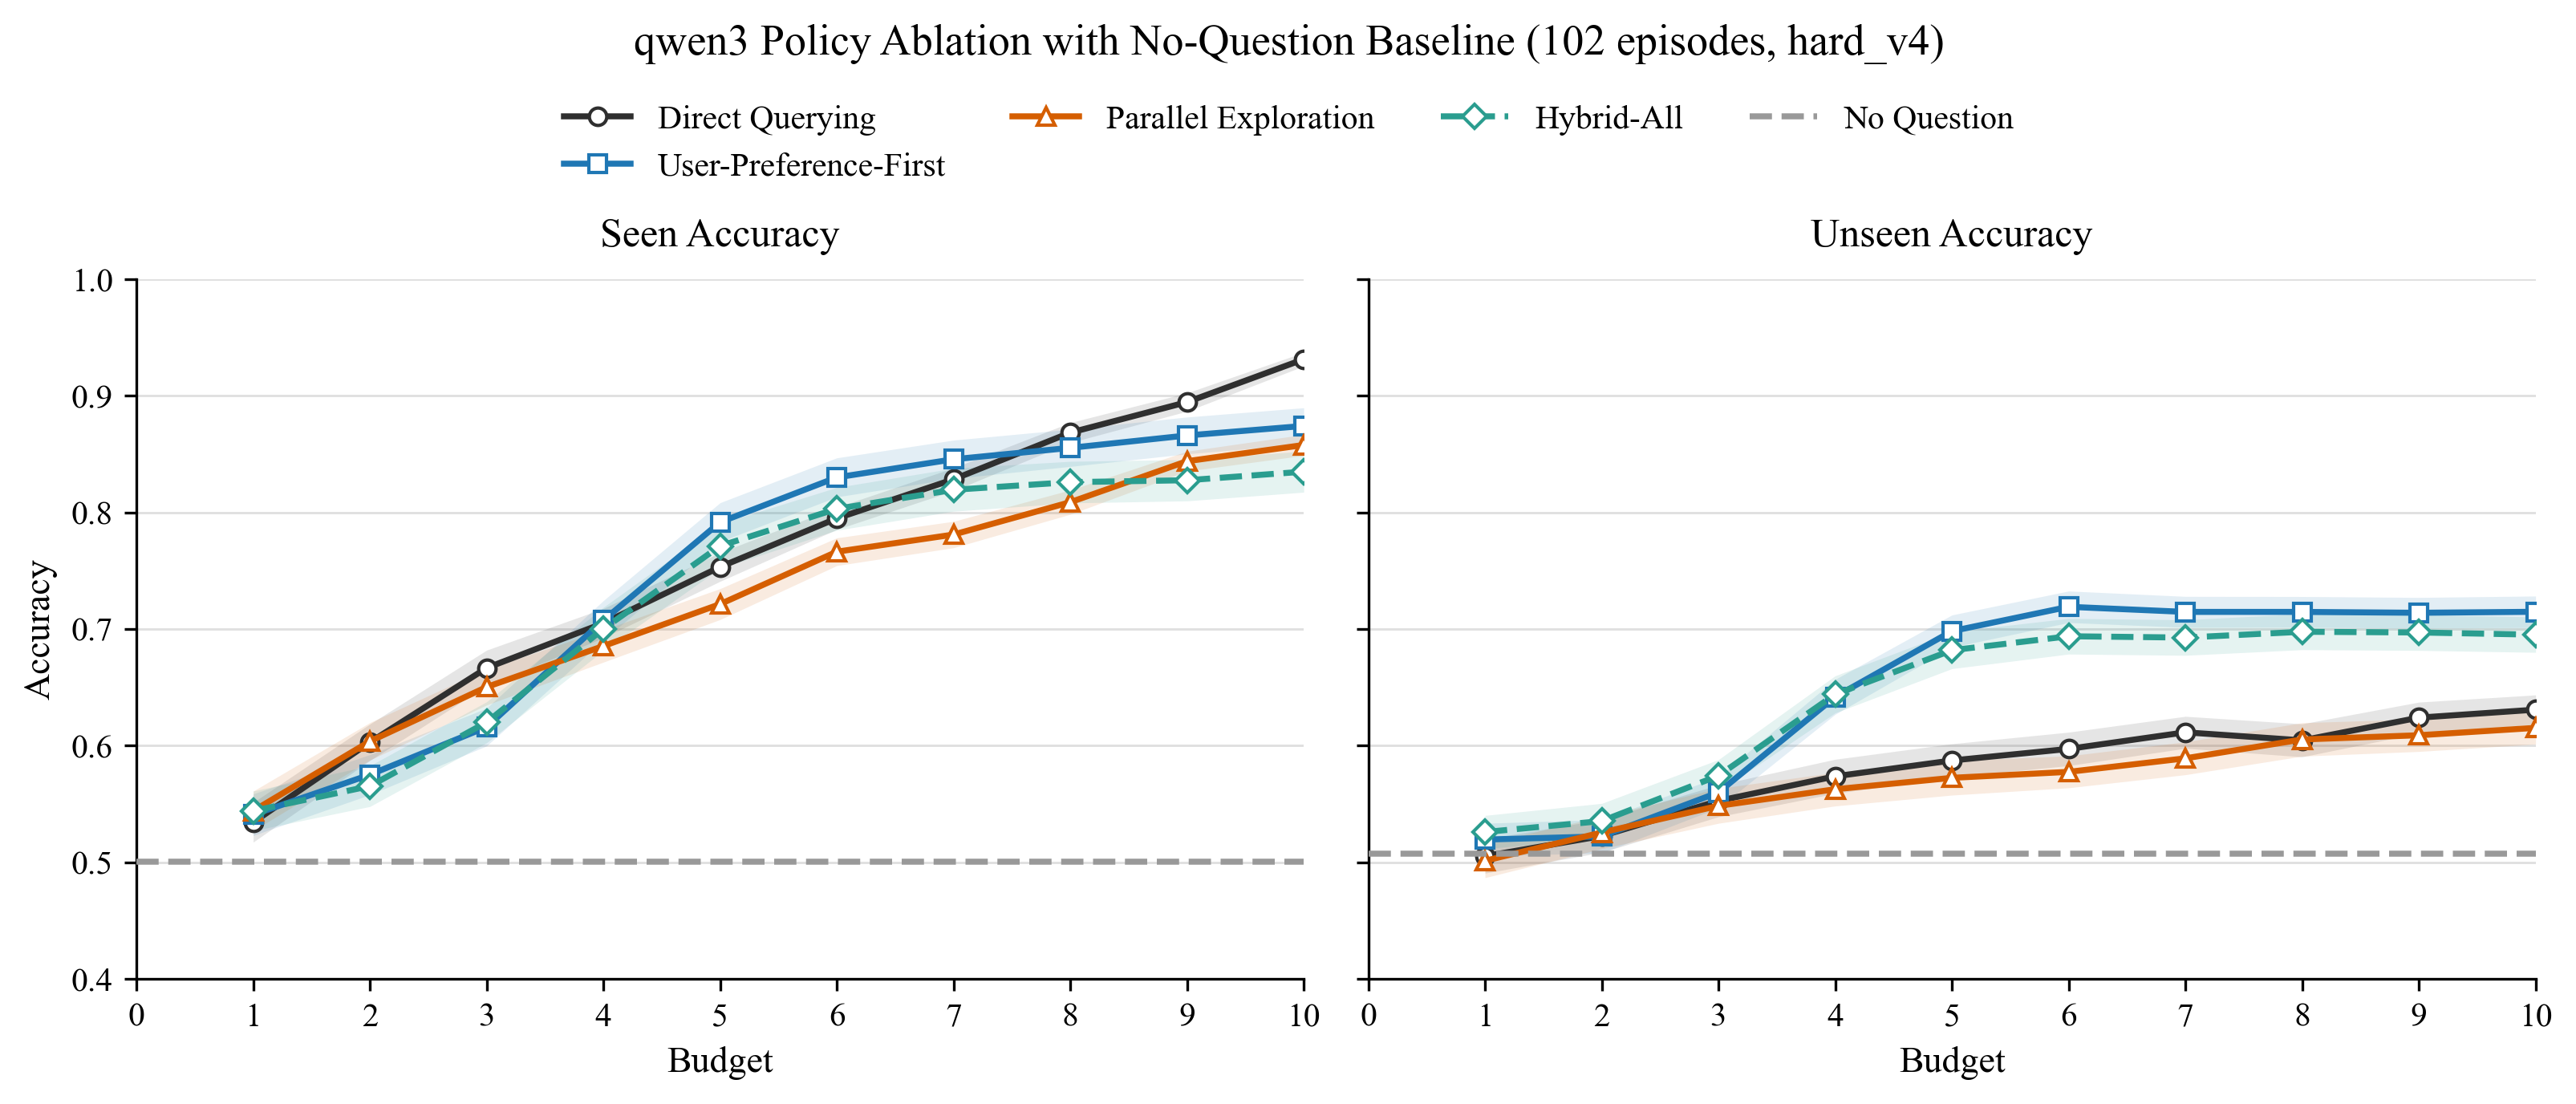
\includegraphics[width=0.9\textwidth]{../plots/qwen3_ablation_with_no_question.png}
  \caption{Seen (left) and unseen (right) accuracy as a function of question budget for four strategies and the No Question baseline (dashed line). Model: Qwen3-8B, 102 episodes. Error bands show $\pm$1 SE.}
  \label{fig:ablation-curves}
\end{figure*}

\subsubsection{Hypothesis Testing}

\textbf{H1 (Monotonic improvement).} All four strategies show monotonically increasing seen accuracy with budget, confirming H1. DQ achieves the steepest seen-accuracy gain (from .534 at $B=1$ to .931 at $B=10$), as expected from a strategy that directly resolves one object per question.

\textbf{H2 (PE-based $>$ DQ on unseen).} UPF achieves .698 unseen accuracy at $B=5$ versus DQ’s .587---a gap of +11.1 percentage points. This advantage emerges at $B \geq 3$ and remains stable through $B=10$ (.715 vs .631, +8.4pp). HYB shows a similar pattern (.682 at $B=5$), confirming that PE-based strategies produce transferable category rules that generalize to unseen objects.
% TODO: Add statistical test (paired t-test or Wilcoxon) with p-values.

\textbf{H3 (PAR $\approx$ DQ on unseen).} PAR achieves .572 unseen accuracy at $B=5$, only marginally above DQ’s .587. At $B=10$, PAR (.615) remains below DQ (.631). This confirms H3: bottom-up induction via PI is structurally less budget-efficient than top-down elicitation via PE, because PI requires multiple AO turns to accumulate evidence before a rule can be proposed.

\textbf{H4 (HYB $\approx$ UPF).} HYB achieves .682 unseen accuracy at $B=5$ versus UPF’s .698, and .695 vs .715 at $B=10$. The differences are small and not statistically significant, confirming H4: adaptive pattern selection does not provide a meaningful advantage over the simpler PE-first heuristic.
% TODO: Add statistical test.

\textbf{H5 (All $>$ No Question).} The No Question baseline achieves .501 seen and .507 unseen accuracy. All strategies at $B \geq 1$ exceed this baseline on seen accuracy, and at $B \geq 3$ on unseen accuracy, confirming H5.

\textbf{H6 (Strategy $>$ Raw LLM).}
% TODO: Fill in when Raw LLM results are available.
\textit{Results pending completion of Raw LLM experiments.}

\subsubsection{Cross-Model Validation}

To verify that the observed patterns are not model-specific, we replicated the No Question baseline with GPT-5-Chat. The No Question baseline with GPT-5-Chat achieves .689 seen and .675 unseen accuracy---substantially higher than Qwen3’s .501/.507, reflecting the stronger commonsense reasoning of the larger model. However, the relative ordering of strategies is expected to remain consistent.
% TODO: Add full GPT-5-Chat ablation results when available.

\subsection{Summary of Findings}

Study~1 establishes three key findings: (1)~PE-based strategies (UPF, HYB) achieve substantially higher unseen accuracy than AO-only or PI-based strategies, demonstrating that top-down preference elicitation produces more transferable organizing rules; (2)~bottom-up induction (PAR) offers no significant advantage over direct querying for generalization, despite its additional complexity; and (3)~adaptive strategy switching (HYB) does not outperform the simpler UPF heuristic. These results provide the first quantitative evidence that questioning strategy choice has a measurable impact on task performance in household preference learning, complementing prior work that has focused primarily on subjective user perceptions.


%% ================================================================
\revend}
%% Study 2: User Study (TODO — to be redesigned and conducted)
%% ================================================================

% TODO: Redesign user study based on Study 1 findings. Key changes from CHI version:
% - Use autonomous system instead of Wizard-of-Oz
% - Include objective performance metrics (placement accuracy)
% - Consider between-subjects design to address fatigue concerns
% - Address reviewer concerns about participant blinding

\section{Study 2: User Study}
\label{sec:study2}

\textit{TODO: Study 2 will evaluate the effects of questioning strategies on user experience and interaction quality with real participants. This section is reserved for future work.}

% Original CHI user study content preserved below for reference:
% ----------------------------------------------------------------
\begin{comment}
\section{User Study}
We conduct an in-person user study (N=18) to examine how varying a robot’s questioning strategy through the QUEST system prompts shapes users’ perceptions and interaction experience in household tasks.

\subsection{Study Design}
We employed a within-subjects design, in which all participants experienced all three task scenarios (\textit{desk tidying}, \textit{office desk tidying}, \textit{bar counter tidying}) and all three questioning strategies (\textit{Direct Querying}, \textit{Parallel Exploration}, \textit{User-Preference-First}). Each participant thus completed nine trials in total, with the order of scenarios and strategies counterbalanced using a Latin square. All scenarios were designed with comparable complexity (approximately 10--12 items and 2--3 storage spaces) to minimize potential confounds. The robot was operated via a Wizard-of-Oz setup to ensure consistent execution across conditions, thereby isolating the effects of the questioning strategies. Figure~\ref{fig:strategies} provides an overview of the three questioning strategies across the three task scenarios.


\begin{figure}[t]
    \centering
    \includegraphics[width=\linewidth]{img/user-study.png}
    \caption{Illustration of the three questioning strategies (\textit{Direct Querying}, \textit{Parallel Exploration}, \textit{User-Preference-First}) across three task scenarios (\textit{study desk tidying}, \textit{office desk tidying}, \textit{bar counter tidying}).}
    \label{fig:strategies}
\end{figure}

\subsection{Tasks}
We design three representative household tidying tasks, each set up as a long-term task with multiple sub-goals and inherent ambiguity. The study is conducted in a lab environment resembling a household setting: the required items (full lists are provided in Appendix~\ref{app:items}) are placed on a central table, and a dual-arm humanoid robot is positioned next to it. Participants’ goal is not to complete the tasks themselves but to \textit{teach the robot} how to perform them. A task is considered complete once the robot can continue without further questioning.  

\textbf{Study Desk Tidying.} Participants teach the robot to organize a cluttered study desk. The goal is to achieve a neat and usable workspace, while individual preferences differ in how items are categorized or whether frequently used objects remain accessible.  

\textbf{Office Desk Tidying.} Participants teach the robot to tidy a desk piled with various objects. The goal is to obtain a clean working surface, while user preferences vary in book arrangement and the use of storage utilities.  

\textbf{Bar Counter Tidying.} Participants teach the robot to organize a cluttered bar counter. The goal is to achieve a clean and safe layout, while user preferences differ in how tableware is arranged and whether tools remain within reach.  
 
\subsection{Apparatus}
We use a dual-arm humanoid robot system in the study. The robot is controlled by a PC running Linux, and an additional laptop is provided for participants to complete questionnaires. The robot is positioned on one side of the table, with participants seated in a designated chair on the opposite side. The field of view of the robot’s camera is marked on the floor, and participants are instructed to remain outside this area before the study begins.  

The experimenter sits at the control PC with direct access to the robot’s emergency stop button and can start or stop the study tasks at any time. To ensure reliable execution of low-level actions, the robot is teleoperated in real time through a VR interface: the experimenter wears a VR headset and controllers, mapping natural arm and hand movements to the robot to achieve precise and flexible manipulation.  Participants interact with the robot using natural language. A microphone array captures speech, which is transcribed and passed to the questioning and teleoperation system to generate context-aware responses.


 

\subsection{Procedure}
After a general introduction to the study and the robot, participants were informed about the study purpose, potential risks, and their rights, and provided written informed consent. The experimenter also familiarized participants with the experimental environment and objects, and reminded them of essential safety instructions (e.g., keeping a safe distance from the robot and avoiding unexpected contact during its movements). Participants then completed a demographic questionnaire, the Affinity for Technology Interaction scale (ATI), and the Negative Attitudes toward Robots Scale (NARS). 

Before the main study, we conducted a standardized \textit{practice trial} in which participants guided the robot through its active questioning to place a bottle into a box. This familiarized participants with the “robot-asks–user-responds” interaction pattern, including answering clarification questions, explaining preferences, and correcting robot actions. Once participants indicated they were comfortable with the interaction, the main study began.  

In the main study, each participant completed three tidying tasks. For each trial, the experimenter prepared the initial environment, and participants stood near the desk or bar counter while teaching the robot to complete the task by answering its questions. No strict time limit was imposed. After each trial, participants filled out a short questionnaire on a separate computer, after which the environment was reset and switched to another questioning strategy. After completing all three tasks, participants took part in a semi-structured interview focusing on their perceived differences between strategies, their preferences and trade-offs, and whether the robot had accurately captured their preferences.


\subsection{Measures and Analysis}
We administered three questionnaires after each task round. First, we used the original NASA-TLX scale~\cite{hart1988development} to evaluate participants’ perceived workload, covering six dimensions: mental demand, physical demand, temporal demand, effort, performance, and frustration. Second, we adopted the Perceived System Curiosity Scale (PSC)~\cite{conf/chi/LeusmannVB0M25}, which includes three subscales—Explorative Curiosity (PSC-E), Investigative Curiosity (PSC-I), and Social Curiosity (PSC-S)—to capture how participants perceived the robot’s “curious” behavior. We chose PSC because prior HRI studies demonstrated that robots displaying curiosity are often perceived as more engaging, human-like, and enjoyable interaction partners, and users tend to prefer teaching or collaborating with such robots over non-curious ones~\cite{8leusmann2025investigating}. Finally, we used the General Self-Efficacy Scale (GSE)~\cite{schwarzer1995generalized} to assess participants’ confidence and sense of control during the teaching process. By repeating these measures after each round, we were able to track how the three questioning strategies influenced subjective experience across different scenarios.



Besides, we logged the complete interaction history between participants and the robot. Robot-side events were categorized into four activity states—\textit{Ask-Confirm}, \textit{Act}, \textit{Fail}, and \textit{Wait}—from which we derived quantitative metrics. Specifically, we modeled event sequences as row-normalized state-transition matrices to examine policy-dependent procedural dynamics (see Section~6.1.1).

For qualitative feedback, after completing all three task rounds, each participant took part in a semi-structured interview lasting about fifteen minutes. The interview questions focused on their preferences and trade-offs between the questioning strategies, their subjective evaluation of the quality and timing of questions. All interviews were audio-recorded, transcribed, and analyzed thematically using Atlas.ti 5. Two researchers independently coded approximately 20\% of the material, after which the codes were discussed with two additional researchers to develop a unified codebook and thematic framework. The remaining material was coded by one researcher, and the final results were validated through team discussions.


\subsection{Participants}
We recruited 18 participants (15 female, 3 male). To reduce novelty effects and focus the study on perceptions of the interaction rather than the robot itself, we aimed to recruit participants with relatively high technological affinity and, where possible, prior HRI experience. Participants’ mean age was 23.8 years ($SD = 6.1$, $min = 21$, $max = 45$). In terms of education, 2 held a doctoral degree, 11 a master’s degree, and 5 a bachelor’s degree. To capture baseline individual differences, we used the Affinity for Technology Interaction scale (ATI)~\cite{franke2019personal}, with an average score of $M = 3.16$ ($SD = 0.7$). We also administered the Negative Attitudes toward Robots Scale (NARS)~\cite{syrdal2009negative}, measuring participants’ negative attitudes toward (S1) interaction with robots ($M = 1.99$, $SD = 0.53$), (S2) social influence of robots ($M = 3.16$, $SD = 0.7$), and (S3) emotions in interaction with robots ($M = 2.59$, $SD = 0.75$).  Regarding prior experience with robots, 6 participants had interacted with robots more than seven times, 10 had interacted 1–7 times, and 2 had never interacted with a robot. Reported types of robots included robotic arms (5), humanoid robots (8), social robots (6), and household robots such as vacuum cleaners or voice assistants (16).  We additionally recorded participants’ task familiarity on a 7-point scale: they reported a mean frequency of 4.0 ($SD = 1.64$) for tidying desks or organizing items over the past six months, and a mean self-rated proficiency of 4.11 ($SD = 1.57$). This baseline data allowed us to control for differences in everyday experience across the three task scenarios.  


\section{Results}

\subsection{Quantitative Interaction Data Analysis}
We verified that the three prompting policies, when deployed on the VLM-controlled robot, produced distinct interaction dynamics. Two core authors annotated all robot-only event states, yielding 413 sequences for \textit{Direct-Querying}, 253 for \textit{User-Preference-First}, and 373 for \textit{Parallel-Exploration}. Robot-only event sequences were modeled across four states—\textit{Ask-Confirm}, \textit{Act}, \textit{Preference-Elicit}, and \textit{Preference-Confirm} (where \textit{Act} denotes a physical operation by the robot)—as row-normalized 4$\times$4 transition matrices for each Participant $\times$ Policy (Fig.~\ref{fig:transition-matrices}). Following Leusmann et al.’s event-transition procedure~\cite{conf/chi/LeusmannVB0M25}, we conducted a repeated-measures multivariate test (Pillai’s trace) with Policy as the within-subject factor and participant IDs as a random effect, using all matrix elements as dependent variables.  

The multivariate effect of Policy was significant (Pillai’s trace = 0.336, $F$(3,32) = 5.392, $p <$ .001). Holm-corrected post-hoc tests further isolated six diagnostic transitions that differed reliably across policies: \textit{Act$\rightarrow$Ask-Confirm}, \textit{Act$\rightarrow$Preference-Elicit}, \textit{Act$\rightarrow$Preference-Confirm}, \textit{Preference-Elicit$\rightarrow$Act}, \textit{Preference-Elicit$\rightarrow$Preference-Elicit}, and \textit{Preference-Confirm$\rightarrow$Act}. These findings establish systematic, policy-dependent state-transition patterns.  

Inspection of the transition matrices corroborated these statistical results. Compared to \textit{Direct-Querying}, both \textit{User-Preference-First} and \textit{Parallel-Exploration} reduced the \textit{Act$\rightarrow$Ask-Confirm} transition ($-0.56$/$-0.69$) and increased preference-related flows such as \textit{Preference-Elicit$\rightarrow$Act} ($+0.26$/$+0.29$). \textit{Parallel-Exploration} additionally amplified \textit{Act$\rightarrow$Preference-Elicit} ($+0.29$). In contrast, \textit{Direct-Querying} exhibited a tight \textit{Ask-Confirm$\leftrightarrow$Act} loop (0.95/1.00), whereas the other two policies routed actions through preference states and suppressed immediate returns to confirmation (\textit{Act$\rightarrow$Ask-Confirm}: 0.44 and 0.31).  

For robustness, a pooled homogeneity $\chi^2$ test on Laplace-smoothed matrices also rejected the null hypothesis of equality across policies ($\chi^2$ = 465.35, $df$ = 30, $p <$ .001). All substantive claims, however, are based on the unsmoothed individual matrices.  

\textit{Interpretation.} The deployed policies encode qualitatively distinct procedural strategies: \textit{Direct-Querying} favors an immediate confirm$\rightarrow$act$\rightarrow$confirm loop; \textit{User-Preference-First} channels actions through preference elicitation and confirmation; and \textit{Parallel-Exploration} interleaves acting with preference-related questioning. These patterns demonstrate that the policies achieved clear behavioral separation when executed on the robot, rather than merely reflecting superficial prompt variations.

\begin{figure}[t]
    \centering
    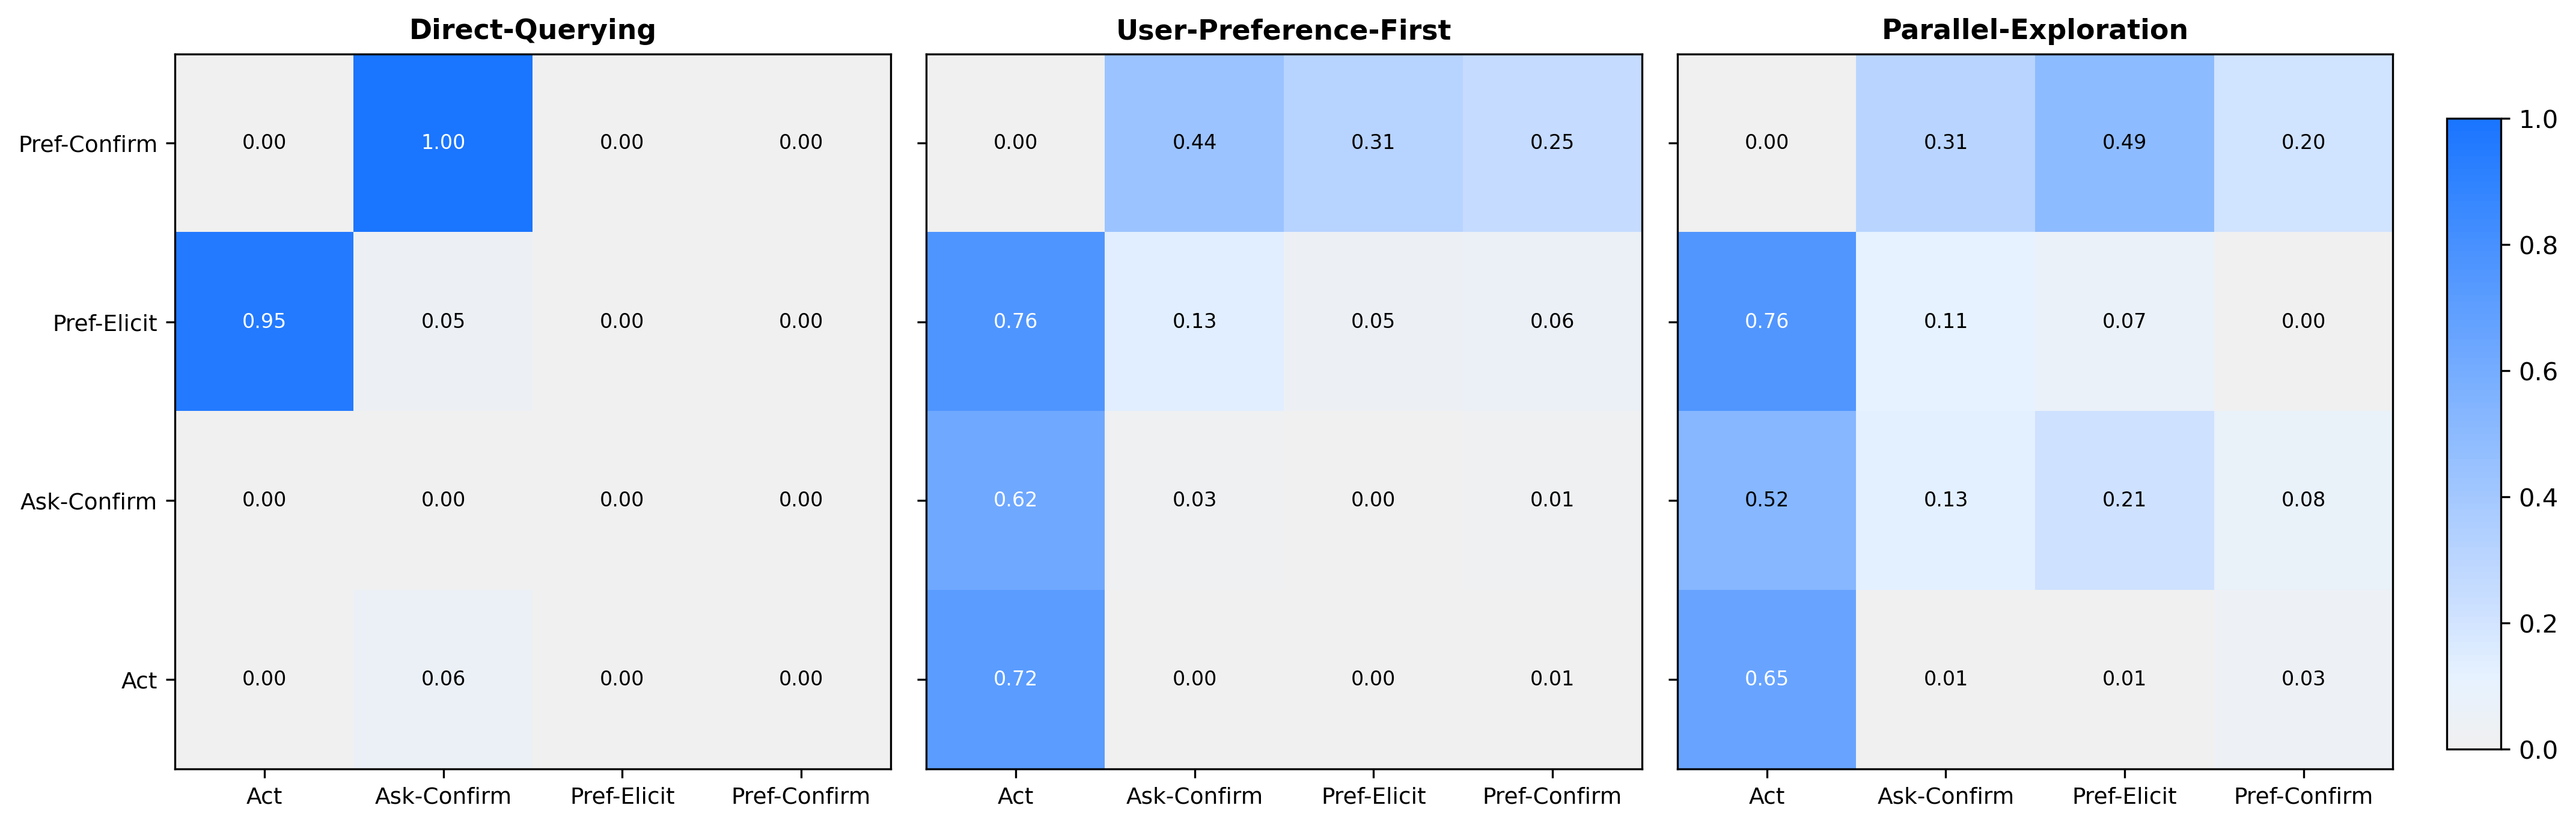
\includegraphics[width=\linewidth]{img/transition-matrices.png}
    \caption{Row-normalized state-transition matrices across the four event states (\textit{Ask-Confirm}, \textit{Act}, \textit{Preference-Elicit}, \textit{Preference-Confirm}) for each questioning policy. \textit{Direct-Querying} shows a tight \textit{Ask-Confirm$\leftrightarrow$Act} loop, whereas \textit{User-Preference-First} and \textit{Parallel-Exploration} route actions through preference states.}
    \label{fig:transition-matrices}
\end{figure}


\subsection{Questionnaire Results}

\begin{table}[ht]
\centering
\caption{Statistical analysis results of all questionnaires (S1 = Direct Querying, S2 = Parallel Exploration, and S3 = User-Preference-First).}
\begin{tabular}{lccccc}
\hline
Measure & W & $p_{norm}$ & $F$ / $\chi^2$ & $p$ & $\eta^2$ / partial $\eta^2$ \\
\hline
\textbf{GSE} & & & & & \\
GSE & 0.920 & .002 & 0.254 & .777 & .009 \\
\hline
\textbf{PSC} & & & & & \\
PSCE        & 0.940 & .009 & 3.401  & .063 & .167 \\
PSCI        & 0.952 & .030 & 6.838  & $<.01$\textsuperscript{*} & .287 \\
PSCS        & 0.961 & .079 & 7.235  & $<.01$\textsuperscript{*} & .299 \\
PSC         & 0.942 & .011 & 7.597  & $<.01$\textsuperscript{*} & .309 \\
\hline
\textbf{NASA-TLX} & & & & & \\
Mental demand   & 0.922 & .002 & 6.644  & $<.05$\textsuperscript{*} & .185 \\
Physical demand & 0.813 & .000 & 0.821  & .663 & .023 \\
Temporal demand & 0.873 & .000 & 1.163  & .559 & .032 \\
Performance     & 0.916 & .001 & 0.982  & .612 & .027 \\
Effort          & 0.940 & .010 & 12.516 & $<.01$\textsuperscript{*} & .348 \\
Frustration     & 0.899 & .000 & 7.609  & $<.05$\textsuperscript{*} & .211 \\
NASA-TLX        & 0.962 & .640 & 4.515  & $<.05$\textsuperscript{*} & .210 \\
\hline
\end{tabular}
\end{table}

\subsubsection{Raw NASA-TLX}
We first tested the normality of the overall NASA-TLX scores. The results indicated that the data under all three strategy conditions followed a normal distribution (Shapiro–Wilk, $p > .05$). Therefore, we conducted a repeated-measures ANOVA. The analysis revealed a significant main effect of strategy on the overall workload ($F(2,34) = 4.52, p < .05$, partial $\eta^2 = .21$), suggesting that different strategies influenced participants’ perceived workload.

We then examined the six subscales separately. Since most of them did not satisfy the normality assumption, we applied non-parametric Friedman tests. The results showed significant effects of strategy on Mental Demand ($\chi^2(2) = 6.64, p < .05$), Effort ($\chi^2(2) = 12.52, p < .01$), and Frustration ($\chi^2(2) = 7.61, p < .05$). In contrast, no significant differences were observed for Physical Demand ($\chi^2(2) = 0.82, p = .663$), Temporal Demand ($\chi^2(2) = 1.16, p = .559$), or Performance ($\chi^2(2) = 0.98, p = .612$).


\begin{figure*}[t]
    \centering
    \begin{subfigure}{0.14\linewidth}
        \centering
        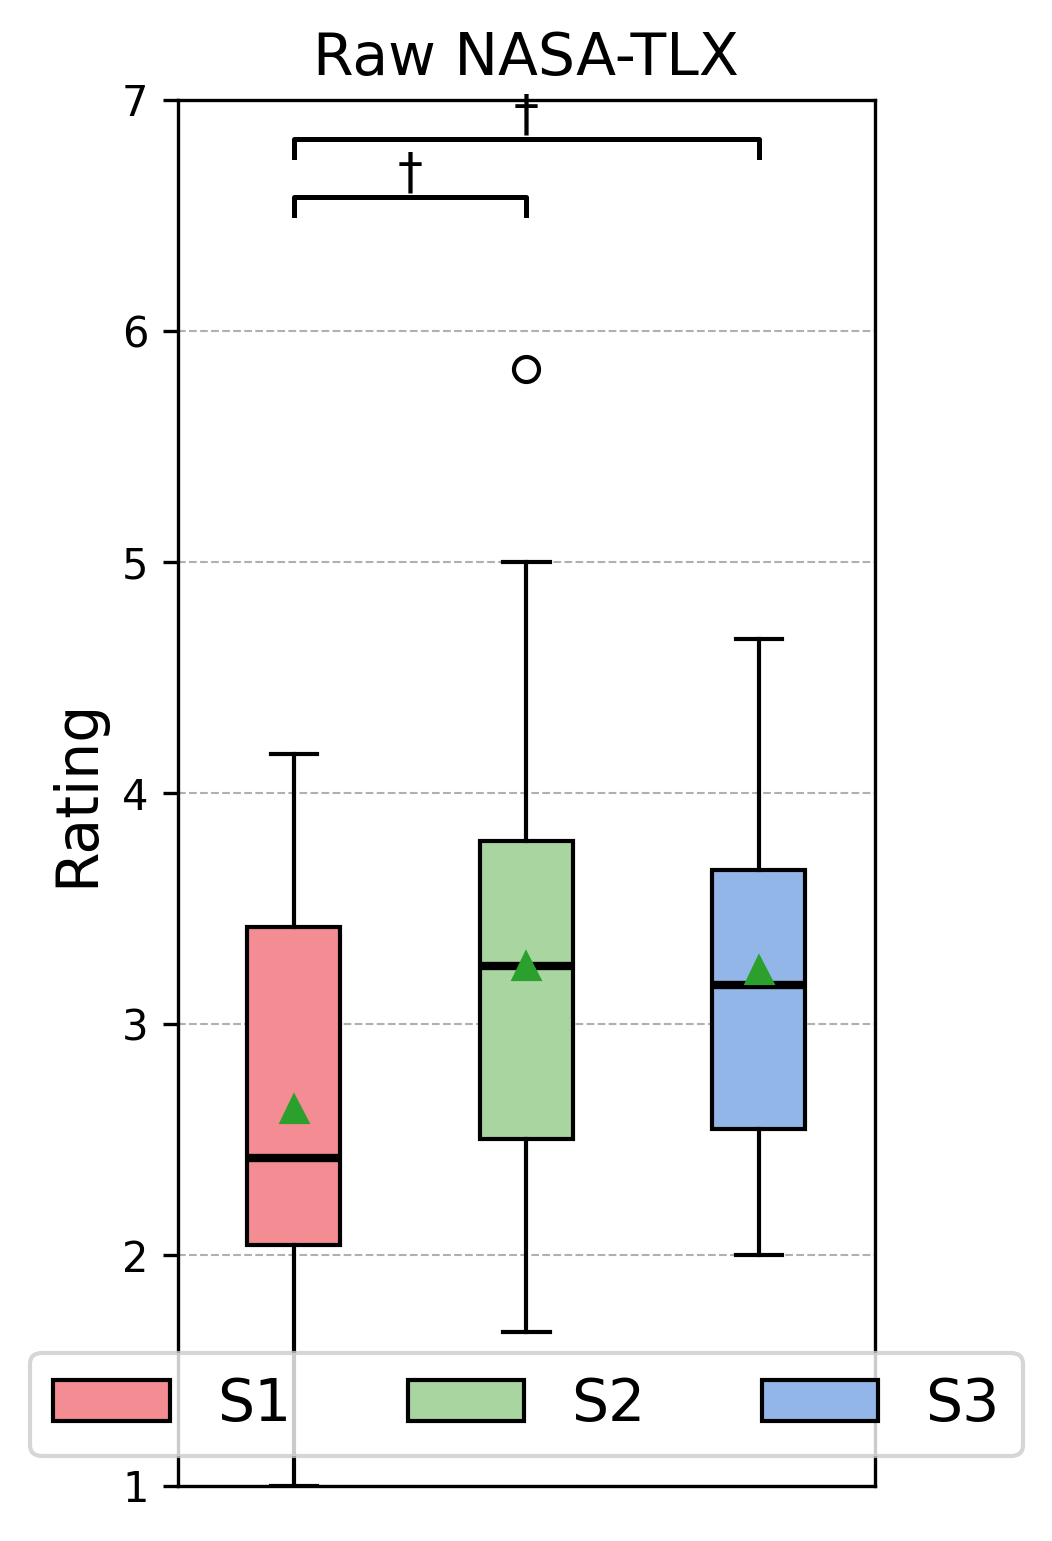
\includegraphics[height=4.7cm]{img/nasa_tlx.png}
        \caption{Raw NASA-TLX}
    \end{subfigure}
    \hfill
    \begin{subfigure}{0.58\linewidth}
        \centering
        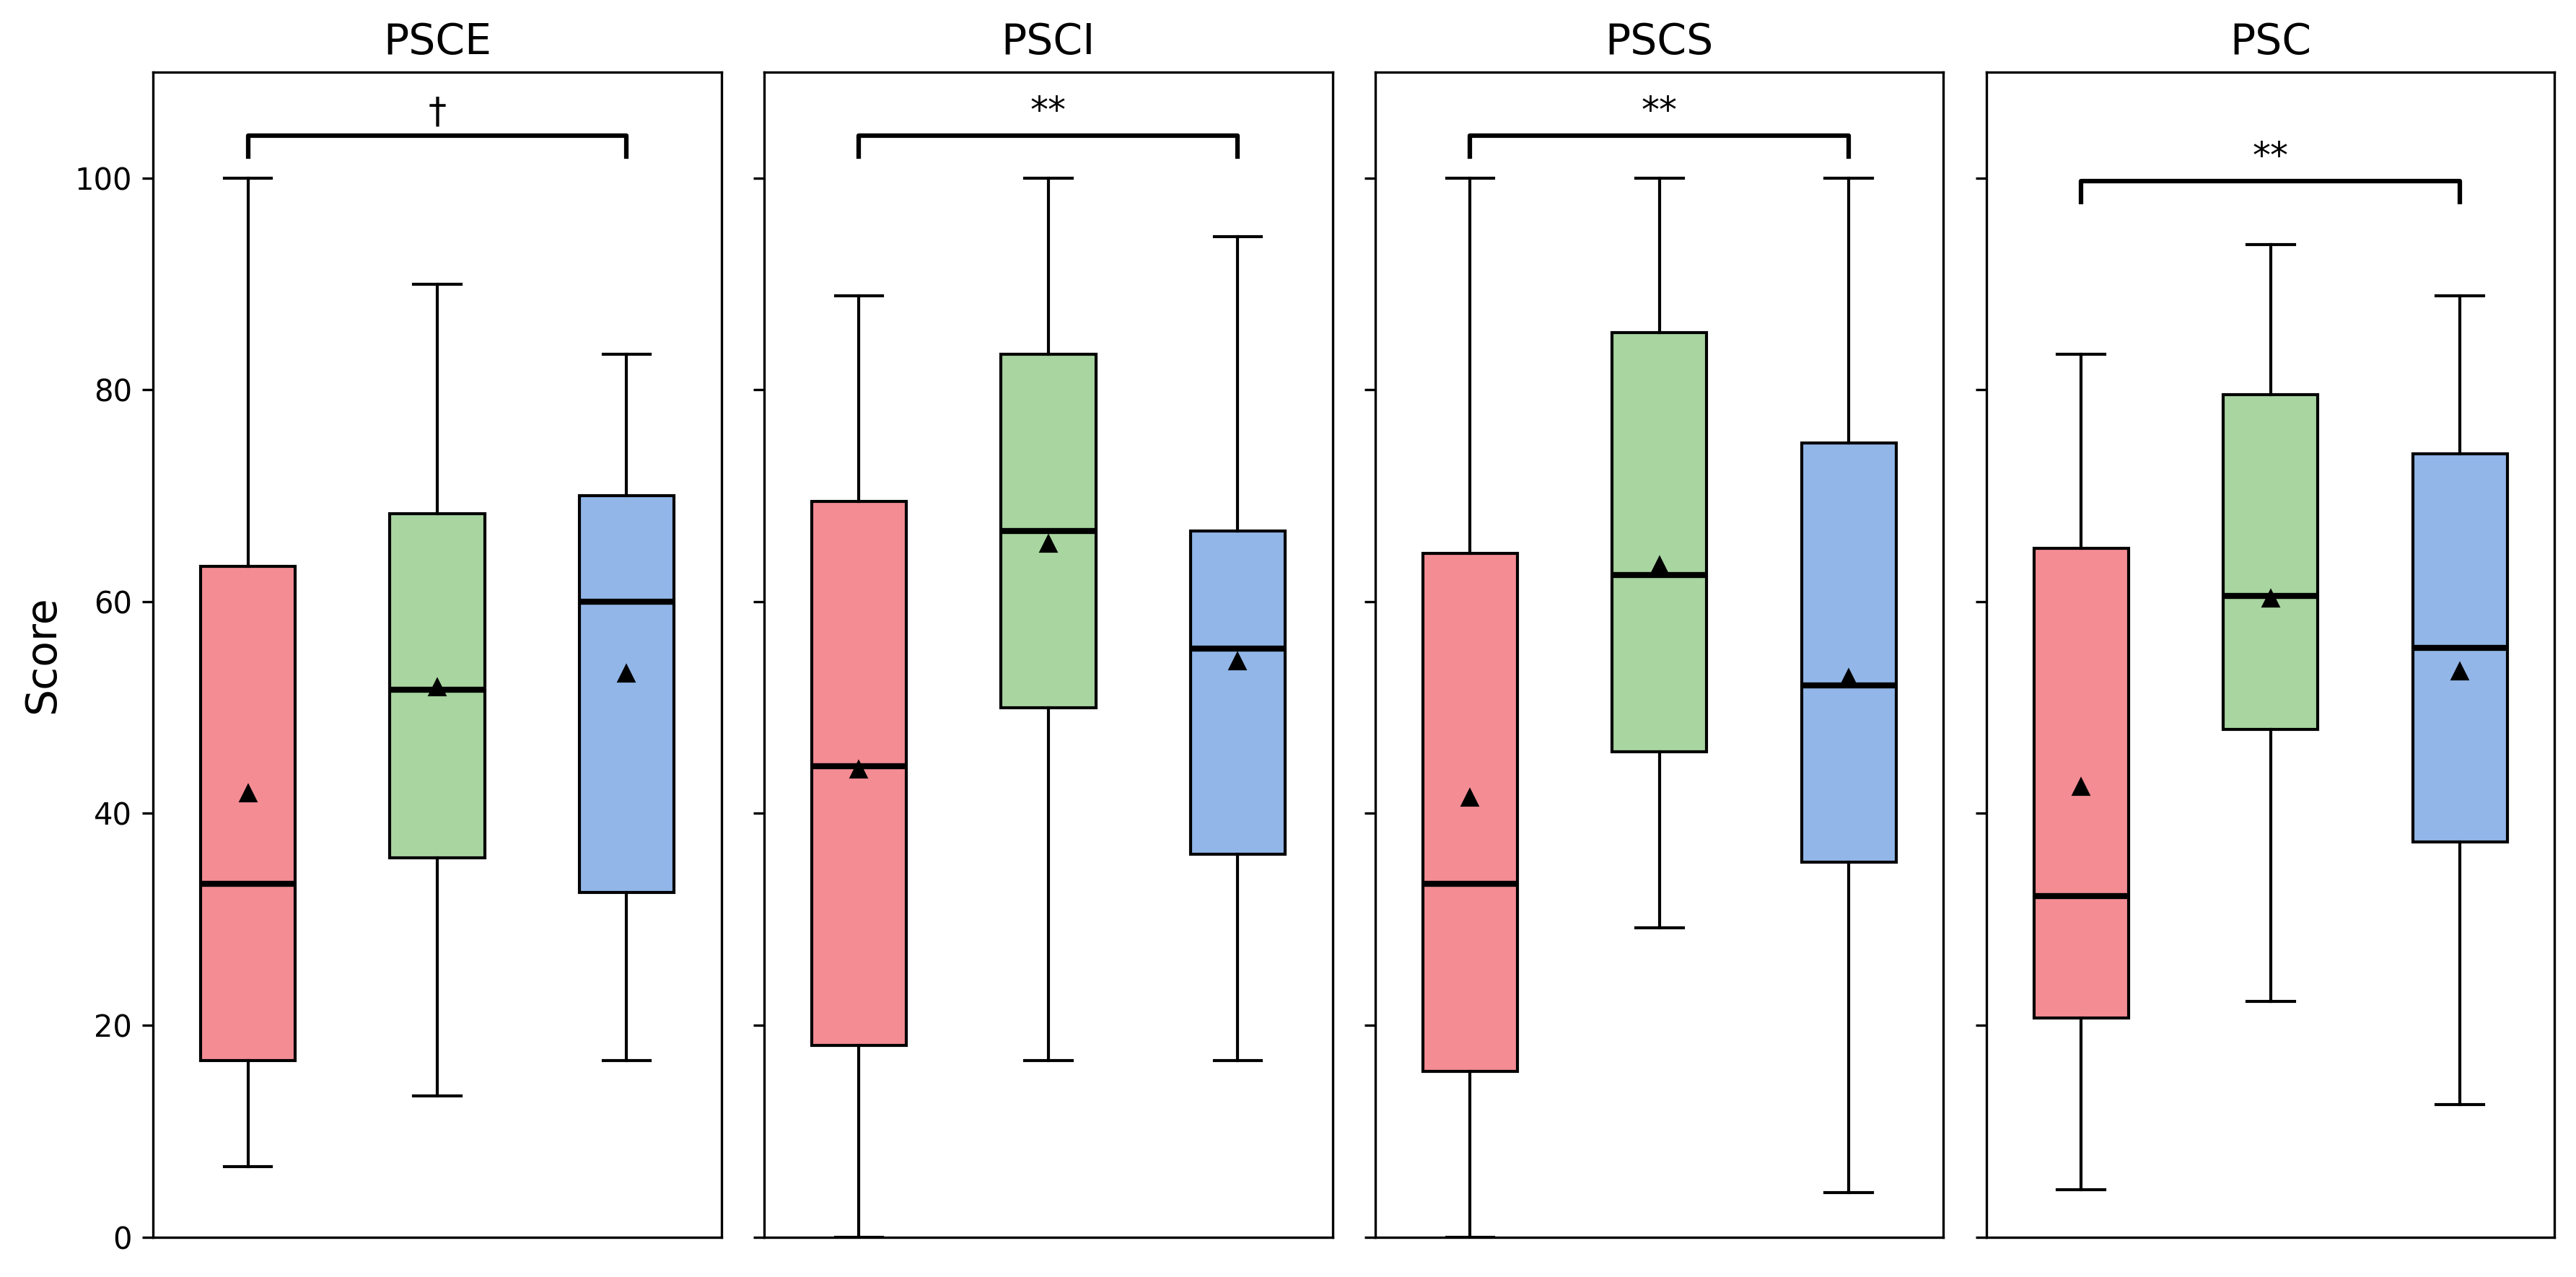
\includegraphics[height=4.7cm]{img/psc.png}
        \caption{PSC scales}
    \end{subfigure}
    \hfill
    \begin{subfigure}{0.12\linewidth}
        \centering
        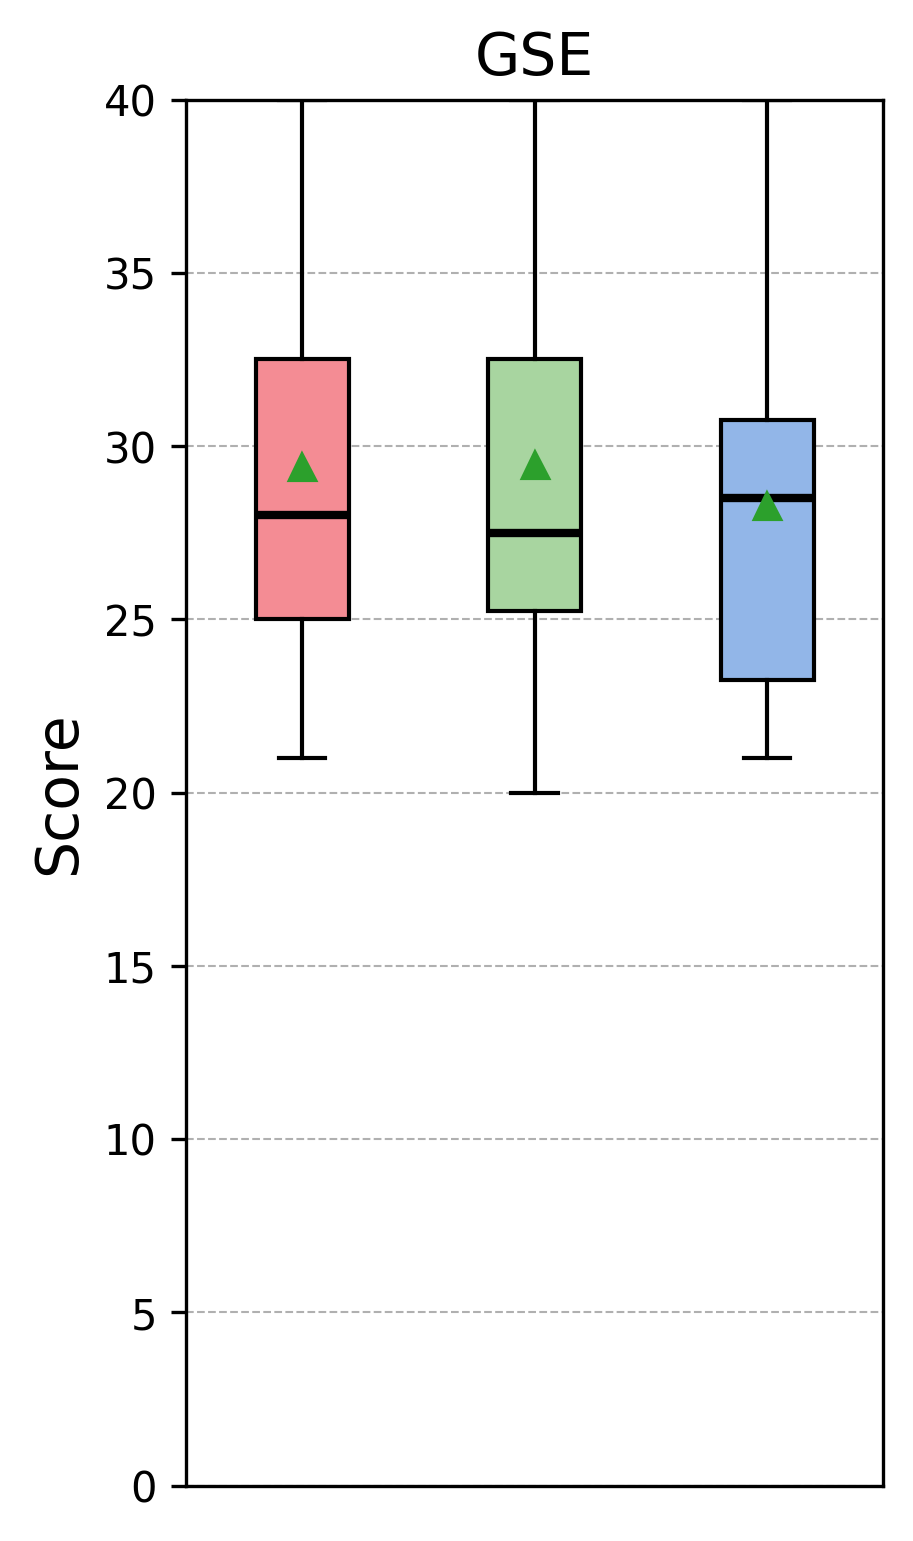
\includegraphics[height=4.7cm]{img/gse.png}
        \caption{GSE}
    \end{subfigure}
    \caption{Subjective measures across strategies: (a) overall workload (NASA-TLX), (b) perceived system curiosity (PSC subscales), and (c) general self-efficacy (GSE). S1 = Direct Querying, S2 = Parallel Exploration, and S3 = User-Preference-First}
\end{figure*}


\subsubsection{PSC}
We conducted normality tests on the scores of the Perceived System Curiosity (PSC) subscales. PSCE ($p = .009$) and PSCI ($p = .030$) deviated from normality, whereas PSCS ($p = .079$) and the overall PSC score ($p = .011$) satisfied the assumption of normality. Since several subscales violated normality assumptions, we employed repeated-measures ANOVA with Greenhouse--Geisser correction where appropriate. The results revealed significant effects of strategy on PSCI ($F(2,34) = 6.838, p < .01, \eta^2 = .29$), PSCS ($F(2,34) = 7.235, p < .01, \eta^2 = .30$), and the overall PSC score ($F(2,34) = 7.597, p < .01, \eta^2 = .31$). Expressive Curiosity (PSCE) only showed a marginal effect ($F(2,34) = 3.401, p = .063, \eta^2 = .17$). Pairwise comparisons further indicated that Strategy~2 yielded significantly higher scores than both Strategy~1 and Strategy~3 on PSCI, PSCS, and the overall PSC, while no significant differences were found between S1 and S3. 


\subsubsection{GSE}
For the General Self-Efficacy Scale (GSE), we first tested the normality of the overall scores. The results indicated a significant deviation from normality (Shapiro--Wilk, $W = 0.920, p = .002$). Since the homogeneity of variance assumption was satisfied (Levene’s test, $p = .973$), we conducted a Welch ANOVA to compare the three strategy conditions. The analysis showed no significant main effect of strategy on the overall GSE scores ($F(2,33.92) = 0.254, p = .777$, $\eta^2 \approx .009$). These findings suggest that the different strategies did not significantly influence participants’ general self-efficacy.


\subsection{Interview Results}

\textbf{Perceptual Differences Between Strategies}
When initiating the interviews, we asked all participants about the differences between the three strategies. \strategy{Parallel Exploration} was considered the most intelligent and efficient strategy by approximately 65\% of participants, capable of summarizing their preferences through a certain degree of interaction and effectively completing tasks. \smallitalic{"Parallel Exploration can infer my preferences based on my feedback, making it more efficient to organize."} \smallitalic{(P13)} In contrast, \strategy{Direct Querying} was perceived as mechanical by about 70\% of participants. \smallitalic{"Direct Querying asks for item locations one by one every time."} \smallitalic{(P08)} This was attributed to the strategy's repetitive questioning about item locations.
For \strategy{User-Preference-First}, approximately 60\% of participants perceived that this strategy inquired about user preferences at the beginning of the conversation and then categorized items based on those preferences.
\begin{quote}
\smallitalic{"User-Preference-First seems to ask general directional questions at first, and after finding a pattern, it starts asking about the relevance between pairs of items."} \smallitalic{(P17)}
\end{quote}

\textbf{Most Liked Strategy}
\strategy{Parallel Exploration} was the most popular strategy, chosen as the favorite by approximately 80\% of participants. The reason for this was its ability to efficiently summarize preferences and quickly provide personalized service:
\begin{quote}
\smallitalic{"Parallel Exploration allows me to complete the task in a shorter time because it can provide personalized recommendations based on my preferences."} \smallitalic{(P05)}
\end{quote}
Furthermore, one user considered its approach of summarizing patterns by arranging two or three items to be a positive performance: \smallitalic{"This strategy is very proactive, and its proactiveness is encouraging me."} \smallitalic{(P04)}
Approximately 15\% of participants chose \strategy{User-Preference-First} as their favorite strategy, primarily because it could summarize participants' preferences and make decisions based on them: \smallitalic{"User-Preference-First summarized my preferences. Although sometimes slower, it closely matches my needs."} \smallitalic{(P06)}
Although \strategy{Direct Querying} was less popular than \strategy{Parallel Exploration} and \strategy{User-Preference-First}, approximately 5\% of participants still considered it an effective strategy, especially for simpler tasks: \smallitalic{"Although Direct Querying is simple and direct, it is still effective when I only need simple categorization."} \smallitalic{(P12)}

\textbf{Least Liked Strategy}
\strategy{Direct Querying} was the most unpopular strategy, with about 70\% of participants considering it their least favorite. Its excessively high query frequency and lengthy interaction time led participants to generally perceive it as inefficient: \smallitalic{"Direct Querying requires me to answer each question individually. Although fast, it makes me feel repetitive and tedious."} \smallitalic{(P12)} The second least favorite was \strategy{User-Preference-First}. Although it could summarize preferences, the summarization process was slow: \smallitalic{"User-Preference-First although it can summarize my preferences, it takes a long time to process, often affecting my task progress."} \smallitalic{(P10)} Additionally, about 50\% of participants believed its summaries lacked accuracy, with one user even finding it aggressive: 
\begin{quote}
\smallitalic{"He is conscious and deliberately trying to explore my preferences, which makes me feel very aggressive."} \smallitalic{(P16)}
\end{quote}
For \strategy{Parallel Exploration}, only a small portion of participants found that: \smallitalic{"It sometimes gives incorrect classifications, which bothers me a bit."} \smallitalic{(P03)}

\textbf{Balancing Efficiency and Effectiveness}
\strategy{Parallel Exploration} was better at balancing effectiveness and efficiency, which was almost a consensus among most participants. \smallitalic{"Parallel Exploration not only provides personalized organization methods but is also more efficient and accurate in task execution."} \smallitalic{(P14)} In contrast, \strategy{Direct Querying} only asked about the placement of single items each time and did not group items according to participant preferences. It offered a more linear thought process that improved better outcomes: \smallitalic{"Direct Querying is good because it's very direct and clearly asks me where to put items."} \smallitalic{(P01)} However, its efficiency was low, making it the least efficient query method among the three strategies. \strategy{User-Preference-First} was pointed out by users for its low execution efficiency and inaccurate summarization process:
\begin{quote}
\smallitalic{"User-Preference-First can indeed summarize my preferences, but it is slow in processing and sometimes summarizes inaccurately, causing me to waste time."} \smallitalic{(P03)}
\end{quote}

\textbf{Teaching Confidence}
Most participants showed high confidence in \strategy{Parallel Exploration}, especially when it could summarize their preferences and execute tasks efficiently. P11 mentioned: \smallitalic{"Parallel Exploration can quickly summarize my preferences and complete tasks, so I have high confidence in it."} In contrast, confidence in \strategy{Direct Querying} and \strategy{User-Preference-First} was lower, particularly for \strategy{Direct Querying} which did not summarize participant preferences: \smallitalic{"Although Direct Querying is fast, I can't trust it because it doesn't summarize my preferences."} \smallitalic{(P18)}

\textbf{Interaction Burden}
Participants felt a heavier interaction burden with \strategy{Direct Querying} because the robot frequently asked for the placement of each item. Approximately 65\% of participants believed \strategy{Direct Querying} increased the cognitive load of the task, making participants feel troubled. P17 mentioned: \smallitalic{"Direct Querying requires me to answer every question each time, which is really stressful. Parallel Exploration makes it much easier for me."} \strategy{Parallel Exploration} and \strategy{User-Preference-First}, on the other hand, placed less pressure on participants in this regard because their query frequencies were significantly reduced, and they could even process items in batches based on their common attributes, further reducing the user's interaction burden.

\textbf{Situational Suitability}
In scenarios requiring explicit item order and position, \strategy{Direct Querying} might be more suitable as it clarifies the location of each item individually, avoiding confusion. This includes unfamiliar contexts, such as temporary accommodations, where personal preferences might not apply:
\begin{quote}
\smallitalic{"For example, going to a hotel by chance, or going for a picnic, or something like that. Then the placement of certain items may not follow the pattern of my long-term preferences. Such scenarios would be more suitable for Direct Querying."} \smallitalic{(P09)}
\end{quote}
It is also preferred in situations where high user control is needed to prevent unwanted robotic behavior:
\begin{quote}
\smallitalic{"Because I have a cat at home, and I'm afraid it might have some strange understanding and do something weird to the cat, causing my cat to get stressed. In such cases, I hope it constantly confirms every detail with me."} \smallitalic{(P04)}
\end{quote}

\textbf{Future Preference and Long-Term Use}
Users' expectations for future use are that the robot can learn their preferences within a short period and automatically summarize patterns when facing daily tasks, minimizing user disturbance as much as possible. Participants mentioned: \smallitalic{"I hope the robot can quickly adapt to my preferences in daily life. Parallel Exploration can do exactly that; it seems capable of meeting my long-term needs."} \smallitalic{(P14)} This indicates participants' advantages in adaptability and flexibility with \strategy{Parallel Exploration}. In contrast, \strategy{User-Preference-First}'s summarization is too slow, and when facing more complex daily scenarios, participants predict its response will be more sluggish. \strategy{Direct Querying} is too mechanical:
\begin{quote}
\smallitalic{"Especially since it needs to ask me the location of each item every time, it cannot self-adjust based on my preferences like Parallel Exploration."} \smallitalic{(P12)}
\end{quote}





\section{Discussion}
\subsection{User Perception and Differentiation of Strategies}
Our findings indicate that users were able to clearly perceive differences between questioning strategies and form consistent judgments about them. The questionnaire results revealed significant contrasts across conditions: Parallel Exploration was perceived as more “curious,” Direct Querying as mechanical and burdensome, and User-Preference-First as offering some value in inferring preferences but at the cost of efficiency. These outcomes were corroborated by NASA-TLX, where Direct Querying reduced interactional complexity but was associated with redundancy and frustration, while Parallel Exploration increased perceived intelligence and proactivity but also raised cognitive demand. 

Interviews further illuminated these perceptual mechanisms. Most participants described Parallel Exploration as the most intelligent and efficient strategy because it could infer their preferences with limited exchanges, echoing earlier work that links perceived competence with positive robot evaluations~\cite{bartneck2009measurement}. In contrast, Direct Querying was often characterized as “repetitive” and “mechanical,” lacking flexibility—an observation consistent with findings that overly rigid interaction patterns undermine user engagement~\cite{naneva2020systematic}. User-Preference-First was valued for helping establish a categorization framework, but its inaccuracy and slower pace often hindered task progress. Such differences not only reflect strategic variation but also how users construct mental models of the robot: some framed it as a “tool” or “butler,” prioritizing efficiency and execution, while others treated it as a “friend” or even a “child,” expressing patience and willingness to “teach” it over time, in line with prior research on anthropomorphism and role attribution~\cite{de2016almost}. 

Taken together, these findings suggest that participants were able to go beyond noticing surface differences and instead formed distinct interpretations of the three strategies. Parallel Exploration was often understood as a proactive way of inferring preferences, Direct Querying as a rigid and repetitive approach, and User-Preference-First as cooperative but slow. Within our tasks, these distinctions shaped how participants reasoned about the robot’s role and capability, influencing whether they framed it as efficient, mechanical, or in need of guidance.



\subsection{Task and Individual Modulators}
Our study further shows that task characteristics substantially shaped strategy preferences. Familiar tasks led participants to favor direct and minimal questioning to avoid redundancy, whereas unfamiliar or ambiguous situations made exploratory strategies more acceptable. Task frequency and importance also influenced expectations of strategy switching. For everyday chores such as tidying a desk, participants preferred robots to gradually learn general rules and reduce interruptions, while for important tasks such as organizing documents they welcomed step-by-step confirmation for accuracy and control. These observations resonate with prior work showing that user expectations for household robots vary by task familiarity and criticality~\cite{yoo_2024_preferences,bansal_2020_supportive}. They also extend evidence that goal-oriented tasks with well-defined outcomes (e.g., placing a single item) often favor preference-first questioning, while process-oriented tasks requiring multiple interdependent steps (e.g., packing a suitcase) invite ongoing exploration~\cite{hu2025task}. 

Individual traits played an equally critical role. Dominant users emphasized efficiency and control, thus preferring direct strategies. Participants with established organizational rules resisted over-exploration, while others without strong rules appreciated additional probing. Parallel exploration proved particularly divisive: some perceived it as intrusive or “aggressive,” reflecting broader concerns about privacy and boundaries in HRI~\cite{cucciniello2023mind}, whereas others described the robot as “child-like” and expressed patience in teaching it, consistent with findings that anthropomorphism can foster tolerance and trust~\cite{de2016almost}. Such polarized responses explain why our questionnaires did not always reveal significant differences, while interviews exposed more nuanced patterns. 

Finally, participants emphasized the challenges of multi-member households, where different users may hold conflicting expectations—one favoring efficiency and directness, another appreciating exploratory engagement. This highlights the need for personalized memory and multi-user modeling to balance competing demands, in line with emerging research on adaptive and multi-user HRI~\cite{rosenthal2010mixed}. Taken together, these findings suggest that task properties and individual differences jointly modulate strategy preferences, reinforcing the importance of adaptive, user-centered questioning frameworks. 

\subsection{Efficiency, Experience, and Long-Term Trade-offs}
We observed a tension between efficiency and experience. Direct Querying kept workload low but felt repetitive due to item-by-item prompts, whereas Parallel Exploration appeared more intelligent and proactive yet raised cognitive demand as it probed for richer information. These patterns support a conservative querying policy: the system should ask only when the expected value of information outweighs the interruption cost, a classic mixed-initiative principle that aligns with active preference-learning approaches designed to minimize queries while learning user objectives~\cite{biyik2019asking}.

Participants also emphasized that short-term impressions do not capture long-term needs. They wanted the robot to remember household rules, avoid redundant questions in routine contexts, and re-query only when uncertainty genuinely increases. Prior work on long-term HRI highlights the role of gradual personalization and memory in sustaining engagement~\cite{matheus2025long}, and recent results in domestic tidying show that compact preference summaries can generalize across related scenarios~\cite{wu2023tidybot}. Taken together, within our tasks this points to memory-augmented, context-aware strategy switching as a practical path to maintain comfort over time.


\subsection{Bridging the HHI–HRI Gap}
 The gap between human–human (HHI) and human–robot (HRI) questioning is especially salient in domestic contexts. In HHI, people naturally mix explicit questions with subtle cues—pointing, gaze, or shared routines—so that preference elicitation rarely feels repetitive. Robots, by contrast, rely on a narrow communication channel: limited prosody, rigid timing, and a lack of nonverbal signals make even simple questions sound mechanical, particularly during everyday tasks like tidying where efficiency is valued~\cite{mutlu2009footing}. Latency further disrupts the flow of collaboration, leading users to perceive interruptions as unnecessary effort.
 
Memory and uncertainty also create friction. In households, humans build up shared context over time (e.g., where items “usually” belong or which rules are exceptions). Current systems, however, often fail to retain preferences across sessions or to judge when re-asking is worthwhile~\cite{leite2013social,ji2023survey}. As a result, the same strategy that feels exploratory in HHI can feel redundant or inefficient in HRI. Users tolerate one-time clarification but become frustrated when a robot repeatedly asks about obvious or previously answered choices~\cite{ahn2022can}.

To close this gap, questioning strategies must adapt to the domestic setting: improving interaction bandwidth with socially legible cues, while also incorporating memory-augmented, cost-aware policies that minimize repetitive queries and leverage past household knowledge. In this way, robots could elicit preferences when uncertainty is high but otherwise act autonomously, allowing strategies that work in HHI to feel more natural in long-term, everyday HRI.

\subsection{Limitations}
Questioning strategies may change over the course of long-term, life-long interactions. Our short-term controlled study cannot capture how preferences and robot behaviors evolve when interactions extend over weeks or months. Understanding these dynamics will be essential for assessing sustainable impacts on user experience and robot learning. 

The current implementation tested strategies in isolation. For experimental control, human questioning patterns were abstracted into single strategies, but in reality people often mix or switch strategies dynamically. This simplification improves interpretability but reduces ecological validity. Future work should explore how robots can flexibly adjust or combine strategies in real time, balancing efficiency, personalization, and user comfort. 

Evaluation was limited to a single household task. While this ensured comparability across participants, it constrains generalizability. Real-world household environments involve diverse and evolving tasks, where robust performance requires both task-specific adaptation and the ability to generalize across contexts. Future studies should investigate whether the identified strategies support such generalization and transfer. 


\end{comment}
%% ================================================================
%% End of commented-out CHI user study content
%% ================================================================


\section{Discussion}
\label{sec:discussion}
{\revstart

\subsection{Top-Down Elicitation Outperforms Bottom-Up Induction}

The most striking finding from Study~1 is the large unseen-accuracy gap between PE-based strategies (UPF, HYB) and the PI-based strategy (PAR). At $B=5$, UPF achieves 69.8\% unseen accuracy versus PAR's 57.2\%---a difference of +12.6 percentage points. This gap arises from a fundamental asymmetry in budget efficiency: a single PE question can discover a category-level rule that immediately generalizes to multiple seen and unseen objects, whereas PI requires multiple prior AO turns to accumulate the evidence needed to propose a testable hypothesis. In practice, PAR spends most of its budget on evidence gathering (AO) and only occasionally triggers PI, resulting in a profile that closely resembles DQ.

This finding has implications for the design of questioning strategies in interactive robot learning: when the goal is to maximize generalization under a limited question budget, top-down preference elicitation should be prioritized over bottom-up induction.

\subsection{The Value of Structured Preference State}

% TODO: Expand this section once Raw LLM results are available.
The comparison between strategy-based approaches and the Raw LLM baseline is designed to isolate the contribution of structured preference state. While the Raw LLM baseline uses the same underlying language model, it lacks the structured state representation ($\mathcal{A}^+$, $\mathcal{P}^+$, $\mathcal{A}^-$) and the evidence-based Final Placement Planner. \textit{Quantitative results for this comparison are pending completion of the Raw LLM experiments.}

We hypothesize that the structured state provides two advantages: (1)~it prevents information loss by explicitly recording confirmed evidence, whereas raw dialogue history is susceptible to LLM context limitations and hallucination; and (2)~it enables the planner to apply evidence hierarchically (preferences $>$ analogies $>$ commonsense), which is difficult to enforce through prompt instructions alone.

\subsection{Budget Efficiency and Diminishing Returns}

UPF's unseen accuracy curve exhibits a characteristic ``elbow'' pattern: rapid improvement from $B=3$ to $B=5$ (from .560 to .698), followed by diminishing returns from $B=5$ to $B=10$ (.698 to .715). This suggests that 3--5 well-chosen PE questions suffice to discover the major organizing rules for a typical household episode. Beyond this point, additional questions contribute mainly to seen-object resolution rather than generalizable preference learning.

This finding supports a \textit{conservative querying policy}: robots should minimize the number of questions asked while maximizing information gain per question---a principle consistent with active preference learning approaches that balance task performance against interruption cost~\cite{biyik2019asking}.

\subsection{Limitations}

\paragraph{Simulated oracle.} Study~1 uses an LLM-based oracle rather than real human participants. While the oracle generates natural-language responses grounded in annotator notes, it may not capture the full variability of human answers (e.g., irrelevant tangents, ambiguous phrasing, or emotional responses). A user study with real participants is needed to validate these findings.

\paragraph{Single domain.} All experiments are conducted in the household rearrangement domain. While the structured preference state and strategies are domain-general in design, empirical validation in other task domains (e.g., cooking assistance, workspace organization) remains future work.

\paragraph{Model dependence.} Results may vary across different LLM backbones. Our cross-model validation with GPT-5-Chat suggests that the No Question baseline performance is model-dependent, but the relative ordering of strategies is expected to be robust.
% TODO: Confirm with full GPT-5-Chat ablation results.


\revend}
\section{Conclusion}
\label{sec:conclusion}
{\revstart

This work investigated how different questioning strategies affect robot learning of household preferences through active dialogue. We make three contributions:

First, through a formative human--human study, we identified three distinct questioning patterns---Direct Querying, Parallel Exploration, and User-Preference-First---confirming that people naturally employ different information-gathering strategies when teaching household tasks (RQ1).

Second, we designed a structured preference learning framework that formalizes these patterns as three questioning design patterns (AO, PE, PI) composed into four questioning strategies (DQ, UPF, PAR, HYB), supported by a structured preference state and evidence-based placement planner (RQ2).

Third, through a large-scale simulation study (102 episodes, 10 budget levels), we demonstrated that questioning strategy choice has a measurable impact on objective task performance: UPF achieves 69.8\% unseen accuracy at budget~5 versus DQ's 58.7\%, a gap of +11.1 percentage points driven by the superior generalizability of top-down preference elicitation (RQ3). We further showed that bottom-up induction (PAR) offers no significant advantage over direct querying, and that adaptive strategy switching (HYB) does not outperform the simpler PE-first heuristic.

% TODO: Add Study 2 contribution when available.

These findings provide the first quantitative evidence that questioning strategies in robot Learning by Asking produce measurable differences in task performance, complementing prior work that has focused primarily on subjective user perceptions. Our results suggest that robots tasked with learning household preferences should prioritize top-down preference elicitation over item-by-item querying, particularly when the question budget is limited.
\revend}
%%
%% The next two lines define the bibliography style to be used, and
%% the bibliography file.
\bibliographystyle{ACM-Reference-Format}
\bibliography{sample-base}


%%
%% If your work has an appendix, this is the place to put it.
\appendix

\section{K-type Categories}
\begin{table}[htbp]
\centering
\caption{K-type category \cite{10.1145/3568294.3580077}}
\label{tab:k-type}
\begin{tabular}{lll}
\hline
\# & Categories     & Description \\
\hline
K1  & Identity         & Information about who or what a person or thing is \\
K2  & Class            & Inclusion relationships of categories \\
K3  & Attributes       & Properties or features of the object \\
K4  & Quantities       & Quantitative specifications \\
K5  & Spatial layout   & Spatial relations among entities \\
K6  & Temporal relation& Temporal information or sequences \\
K7  & Contents         & Additional detailed information \\
K8  & Procedure        & Order or method of a specific process \\
K9  & Causality        & Causal chains of events or states \\
K10 & Intention        & Motivation, aim or plan of another agent \\
K11 & Internal state   & Mental states such as preference or mood of another agent \\
\hline
\end{tabular}
\end{table}



\section{Task Materials and Layouts}
\label{app:items}

Figure~\ref{fig:layouts} shows the initial setups of the three tidying tasks. Each setup included 10--12 items distributed across a central table and 2--3 designated storage areas. The object composition and spatial layout were carefully designed to be comparable in complexity while still allowing for individual variation in preferences (e.g., categorization, accessibility, or arrangement).  

\begin{figure}[t]
    \centering
    \includegraphics[width=\linewidth]{img/layout_1.png}
    \caption{Initial layouts for the three household tidying tasks: bar counter(left), study desk (middle), and office desk(right). Each scenario contains approximately 10--12 items and 2--3 storage spaces, designed with comparable complexity while preserving room for individual preferences.}
    \label{fig:layouts}
\end{figure}


\subsection{Item Lists}
\label{app:items}

\begin{table}[h]
\centering
\begin{tabular}{ll}
\toprule
\textbf{Item} & \textbf{Attributes} \\
\midrule
Plate & Black, with white bird pattern \\
Bowl & Small, white, with gold rim \\
Brush & Gray sponge brush on a stick \\
Sauce & Glass jar with red cap \\
Noodles & Instant noodle cup, red and black \\
Detergent & Bottle of yellow dish soap \\
Oil & Glass bottle of cooking oil \\
Spoon & White, ceramic \\
Sponge & Yellow, wavy shape \\
Sponge & Yellow, wavy shape \\
Lemon & Yellow, whole fruit \\
\bottomrule
\end{tabular}
\caption{Bar counter tidying item list.}
\end{table}

\begin{table}[h]
\centering
\begin{tabular}{ll}
\toprule
\textbf{Item} & \textbf{Attributes} \\
\midrule
Bottle & Transparent, plastic, with green cap \\
Notebook & Cork cover \\
Book & White, pink and green cover \\
Book & White cover, ``Design as Art'' \\
Fan & White, round \\
Measure & Retractable tape measure \\
Tape & Roll of black electrical tape \\
Sunglasses & Brown lenses, black frame \\
Keyboard & Black, Logitech brand \\
Basket & Silver, wire mesh \\
Bin & Blue, plastic \\
Doll & Gray, owl-shaped doll \\
\bottomrule
\end{tabular}
\caption{Office desk tidying item list.}
\end{table}


\begin{table}[h]
\centering
\begin{tabular}{ll}
\toprule
\textbf{Item} & \textbf{Attributes} \\
\midrule
Lamp & White, phone holder style \\
Mouthwash & Transparent bottle with blue \\
Toolset & Orange and transparent \\
Yogurt & White, plastic bottle \\
Baseball & White with red stitching \\
Doll & Brown, bear-shaped doll \\
Tissues & Blue and white package \\
Thermos & Light green \\
Gamecard & Green Xbox game case \\
Gamecard & Black GTA game case \\
Umbrella & Black and white striped \\
Remote & White, air conditioner remote \\
\bottomrule
\end{tabular}
\caption{Study desk tidying item list.}
\end{table}

\end{document}
\endinput
%%
%% End of file `sample-sigconf-authordraft.tex'.
